\documentclass[format=acmsmall,review=false,screen=true]{acmart}

% Metadata Information
%% \acmJournal{TACO}
%% \acmVolume{0}
%% \acmNumber{0}
%% \acmArticle{00}
%% \acmYear{2019}
%% \acmMonth{1}
%% \copyrightyear{2019}
%\acmArticleSeq{9}

% Copyright
%\setcopyright{acmcopyright}
%\setcopyright{acmlicensed}
%\setcopyright{rightsretained}
%\setcopyright{usgov}
%\setcopyright{usgovmixed}
%\setcopyright{cagov}
%\setcopyright{cagovmixed}
\setcopyright{acmcopyright}
\acmJournal{TACO}
\acmYear{2019}
\acmVolume{1}
\acmNumber{1}
\acmArticle{1}
\acmMonth{1}
\acmPrice{}
\acmDOI{10.1145/3355606}

% DOI
%\acmDOI{0000001.0000001}

% Paper history
\received{February 2019}
\received[revised]{June 2019}
\received[accepted]{August 2019}

%% Bibliography style
\bibliographystyle{abbrv}
%\bibliographystyle{ACM-Reference-Format}
%\citestyle{acmnumeric}     %% For numeric citations

\pdfoutput=1 % arXiv

\usepackage{tc}

\usepackage[utf8]{inputenc}
\usepackage{amsmath}
\usepackage{amsfonts}
\usepackage{nicefrac}
\usepackage{microtype}
\usepackage{xspace,url}
%\usepackage{luximono}
\usepackage{etoolbox} % For advanced style overriders
\usepackage{booktabs} % For formal tables
\usepackage{multirow}
\usepackage{relsize}
\usepackage{todonotes}
%\usepackage[hidelinks]{hyperref}

% \usepackage[style=numeric,firstinits=true,%
% backend=biber,maxbibnames=99,sortcites=true,giveninits=true,%
% doi=false,isbn=false,url=false]{biblatex}

% \DeclareSourcemap{
%   \maps[datatype=bibtex]{
%     % anonymize Vasilache2018TC entry
%     \map[overwrite]{
%       \step[fieldsource=entrykey,match={Vasilache2018TC},final]
%       \step[fieldset=author, fieldvalue={Anonymous Author(s)}]
%     }
%   }
% }

\usepackage{array}
\newcolumntype{L}[1]{>{\raggedright\let\newline\\\arraybackslash\hspace{0pt}}m{#1}}
\newcolumntype{C}[1]{>{\centering\let\newline\\\arraybackslash\hspace{0pt}}m{#1}}
\newcolumntype{R}[1]{>{\raggedleft\let\newline\\\arraybackslash\hspace{0pt}}m{#1}}

\newcommand{\ic}[1]{\textrm{\lstinline[language=tc]{#1}}}

\def\topsep{\skip0}
\def\listisep{\skip0}
\def\labelsep{\skip0}

\renewcommand{\subsectionautorefname}{Section}

\newcommand{\tblref}[1]{\autoref{tbl:#1}}

\newcommand{\figref}[1]{Figure~\ref{fig:#1}}
\newcommand{\figreftwo}[2]{Figures~\ref{fig:#1} and~\ref{fig:#2}}
\newcommand{\figrefthree}[3]{Figures~\ref{fig:#1}, \ref{fig:#2} and~\ref{fig:#3}}
\newcommand{\subfiglabel}[1]{\textbf{#1}}
\newcommand{\subfigcap}[1]{\textbf{~~#1}}
\newcommand{\subfigref}[2]{Figure~\ref{fig:#1}#2}

\usepackage[binary-units]{siunitx}
\sisetup{table-number-alignment=center,table-align-text-post=false,group-separator={,}}%table-parse-only

\newenvironment{tab}[2][\linewidth]
{\begin{tabular*}{#1}[t]{@{\extracolsep{\fill}}>{\hspace{4pt}}#2}}%
{\end{tabular*}}

%\AtBeginEnvironment{minted}{\footnotesize} % size for Python listings
% \makeatletter
% \def\mdseries@tt{m}
% \makeatother
% \usepackage{minted}
% \makeatletter
% \def\mdseries@tt{m}
% \makeatother

% Global kill switch to remove all comments
\newif\iffinal
%\finalfalse % Use me to render comments
\finaltrue % Use me to hide comments and issue warnings

% Some colors that should be readable on white BG
% Use for your comments.  Ask Alex for more if necessary.
\definecolor{DarkGreen}{HTML}{33AA33}
\definecolor{OldMauve}{HTML}{673147}
\definecolor{CrimsonRed}{HTML}{990000}
\definecolor{Plum}{HTML}{8E4585}
\definecolor{Sienna}{HTML}{882D17}
\definecolor{Indigo}{HTML}{330088}

% Comment macros.  Please also define an empty macro for \iffinal version.
\iffinal
\newcommand{\wmnote}[1]{\TODO{Billy: #1}}
\newcommand{\acnote}[1]{\TODO{Albert: #1}}
\newcommand{\aznote}[1]{\TODO{Alex: #1}}
\newcommand{\ntvnote}[1]{\TODO{Nico: #1}}
\newcommand{\ttnote}[1]{\TODO{Theo: #1}}
\newcommand{\zdnote}[1]{\TODO{Zach: #1}}
\newcommand{\aanote}[1]{\TODO{Andrew: #1}}
\newcommand{\TODO}[1]{\message{*** TODO #1}}
\else
\newcommand{\wmnote}[1]{{\scriptsize \color{red} [[ Billy: #1 ]]}}
\newcommand{\acnote}[1]{{\scriptsize \color{purple} [[ Albert: #1 ]]}}
\newcommand{\aznote}[1]{{\scriptsize \color{blue} [[ Alex: #1 ]]}}
\newcommand{\ntvnote}[1]{{\scriptsize \color{DarkGreen} [[ Nico: #1 ]]}}
\newcommand{\ttnote}[1]{{\scriptsize \color{CrimsonRed} [[ Theo: #1 ]]}}
\newcommand{\zdnote}[1]{{\scriptsize \color{Sienna} [[ Zach: #1 ]]}}
\newcommand{\aanote}[1]{{\scriptsize \color{Indigo} [[ Andrew: #1 ]]}}
\fi

% Name defines
\newcommand{\ourtoolkitname}{TC\xspace}
\newcommand{\isl}{\textit{isl}\xspace}
\newcommand{\ppcg}{\mbox{PPCG}\xspace}
\newcommand{\rstreamtf}{\mbox{R-Stream$\cdot$TF}\xspace}
\newcommand{\pencil}{\textsc{Pencil}\xspace}

% Math notations
\newcommand{\Ocal}{\mathcal{O}}

\usepackage{tikz}
\usetikzlibrary{decorations.pathreplacing,shapes,arrows,positioning,calc}
\newfont{\subheadfnt}{ptmbi8t at 10pt}
\newcommand{\subheading}[1]{\subsection*{\subheadfnt #1}}

\newenvironment{normalitemize}{\setlength{\labelsep}{0.5em}\begin{itemize}}
                              {\end{itemize}}
\newenvironment{normalenumerate}{\setlength{\labelsep}{0.5em}\begin{enumerate}}
                                {\end{enumerate}}

\tikzset{
  pblock/.style={
    rectangle,
    rounded corners,
    draw=black, thin,
    minimum width=2.2cm,
    inner sep=2pt,
    % outer sep=4pt,
    align=left,
    anchor=west,
    fill=yellow,
    font={\fontsize{9.5}{10.2}\selectfont},
    %font={\ttfamily\fontsize{12}{14}\selectfont},
    text=black,
    draw=gray,
    thick,
    auto,
    node distance=.2cm and .1cm,
  },
  atune/.style={
    ellipse,
    rounded corners,
    draw=black, thin,
    minimum width=2.2cm,
    inner sep=2pt,
    % outer sep=4pt,
    align=left,
    anchor=west,
    fill=green,
    font={\fontsize{9.5}{10.2}\selectfont},
    %font={\ttfamily\fontsize{12}{14}\selectfont},
    text=black,
    draw=gray,
    thick,
    auto,
    node distance=.2cm and .1cm,
  },
  cfedge/.style={
    font=\itshape,
    draw=black,
    ->,
    >=stealth'
  },
  process/.style={
    draw,
    fill=orange!50,
    rectangle,
    minimum height=1.5em,
    minimum width=5em,
    align=center,
    font=\small,
  },
  form/.style={
    draw,
    fill=blue!30,
    ellipse,
    minimum height=1em,
    align=center,
    font=\footnotesize,
  },
  slave/.style={
    execute at end picture={
      \coordinate (lower right) at (current bounding box.south east);
      \coordinate (upper left) at (current bounding box.north west);
      \pgfresetboundingbox
      \path (upper left) rectangle (lower right);
    }
  }
}

\title[The Next 700 Accelerated Layers]{The Next 700 Accelerated Layers: From Mathematical Expressions of Network Computation Graphs to Accelerated GPU Kernels, Automatically}

\author{Nicolas Vasilache}
\affiliation{%
  \institution{Facebook AI Research\footnotemark[2]}
  \city{New York City}
  \country{NY, USA}
}
\email{nicolas.vasilache@gmail.com}
\author{Oleksandr Zinenko}
\affiliation{%
  \institution{Inria and ENS\footnotemark[2]}
  \city{Paris}
  \country{France}
}
\email{oleksandr.zinenko@inria.fr}
\author{Theodoros Theodoridis}
\affiliation{%
  \institution{ETH Z\"{u}rich}
  \city{Z\"{u}rich}
  \country{Switzerland}
}
\email{theodort@student.ethz.ch}
\author{Priya Goyal}
\affiliation{%
  \institution{Facebook AI Research}
  \city{New York City}
  \country{NY, USA}
}
\email{prigoyal@fb.com}
\author{Zachary DeVito}
\affiliation{%
  \institution{Facebook AI Research}
  \city{Menlo Park}
  \country{CA, USA}
}
\email{zdevito@fb.com}
\author{William S.\ Moses}
\affiliation{%
  \institution{MIT CSAIL}
  \city{Cambridge}
  \country{MA, USA}
}
\email{wmoses@mit.edu}
\author{Sven Verdoolaege}
\affiliation{%
  \institution{Polly Labs \& Facebook AI Research\footnotemark[3]}
  \city{Leuven}
  \country{Belgium}
}
\email{skimo@kotnet.org}
\author{Andrew Adams}
\affiliation{%
  \institution{Facebook AI Research\footnotemark[4]}
  \city{Menlo Park}
  \country{CA, USA}
}
\email{andrew.b.adams@gmail.com}
\author{Albert Cohen}
\affiliation{%
  \institution{Inria, ENS and Facebook AI Research\footnotemark[2]}
  \city{Paris}
  \country{France}
}
\email{albert.cohen@inria.fr}

\renewcommand{\shortauthors}{Vasilache, Zinenko, Theodoridis, Goyal, DeVito, Moses, Verdoolaege, Adams, Cohen}

%   Nicolas Vasilache\\
%   \footnotesize Facebook AI Research\\
%   \footnotesize \url{ntv@fb.com}\\
%   \And
%   Theodoros Theodoridis\\
%   \footnotesize ETH Z\"{u}rich\\
%   \footnotesize \url{theodort@student.ethz.ch}\\
%   \AND
%   Priya Goyal\\
%   \footnotesize Facebook AI Research\\
%   \footnotesize \url{prigoyal@fb.com}\\
%   \And
%   Zachary DeVito\\
%   \footnotesize Facebook AI Research\\
%   \footnotesize \url{zdevito@fb.com}\\
%   \And
%   William S. Moses\\
%   \footnotesize MIT CSAIL\\
%   \footnotesize \url{wmoses@mit.edu}\\
%   \AND
%   Sven Verdoolaege\\
%   \footnotesize \hskip-1cm Polly Labs \& Facebook AI Research\hskip-1cm\,\\
%   \footnotesize \url{sven.verdoolaege@gmail.com}\\
%   \And
%   Andrew Adams\\
%   \footnotesize Facebook AI Research\\
%   \footnotesize \url{andrew.b.adams@gmail.com}\\
%   \And
%   Albert Cohen\\
%   \footnotesize \hskip-1cm Inria \& ENS, DI \& Facebook AI Research\hskip-1cm\,\\
%   \footnotesize \url{albert.cohen@inria.fr}

\begin{document}

\renewcommand{\thefootnote}{\fnsymbol{footnote}}
\footnotetext[2]{With Google AI at the time of publication.}
\footnotetext[3]{With Cerebras at the time of publication.}
\footnotetext[4]{With Adobe at the time of publication.}
\renewcommand{\thefootnote}{\arabic{footnote}}

\begin{abstract}
Deep learning frameworks automate the deployment, distribution,
synchronization, memory allocation, and hardware acceleration of
models represented as graphs of computational operators. These
operators wrap high-performance libraries such as cuDNN or
NNPACK. When the computation does not match any predefined library
call, custom operators must be implemented, often at high
engineering cost and performance penalty, limiting the pace of
innovation. To address this productivity gap, we propose and
evaluate: (1) a domain-specific language with a tensor
notation close to the mathematics of deep learning; (2) a
Just-In-Time optimizing compiler based on the polyhedral framework;
(3) carefully coordinated linear optimization and evolutionary
algorithms to synthesize high-performance CUDA kernels; (4) the
transparent integration of our flow into PyTorch and Caffe2,
providing the fully automatic synthesis of high-performance GPU
kernels from simple tensor algebra. The performance is comparable
to, and often exceeds the performance of highly tuned libraries.
\end{abstract}

\keywords{deep learning layers, polyhedral compilation, GPU acceleration.}

\begin{CCSXML}
<ccs2012>
<concept>
<concept_id>10011007.10011006.10011041</concept_id>
<concept_desc>Software and its engineering~Compilers</concept_desc>
<concept_significance>500</concept_significance>
</concept>
</ccs2012>
\end{CCSXML}

\ccsdesc[500]{Software and its engineering~Compilers}

\maketitle

\section{Introduction}

Deep neural networks trained with back-propagation
learning~\cite{Backprop89} are a method of choice to solve complex
problems with sufficient data. Popular graph computation
engines~\cite{Theano,Torch7,MXNet,TensorFlow,PyTorch} offer high-level
abstractions for optimizing and executing deep neural networks
expressed as graphs of tensor operations. These frameworks make
transparent use of heterogeneous computing systems, leveraging
highly-optimized routines for individual operators.  While these
operators are sufficient for many applications, they fall short in a
number of instances.  Developing a novel type of layer or network
architecture incurs high engineering cost or performance penalty.
Even if a new layer may be expressed in terms of existing library
primitives, performance is often far from peak for two reasons: missed
optimizations across operators, and no tuning for its specific
size, shape and data flow~\cite{FBFFT15}.  Our work aims at addressing this
\emph{productivity gap}.\footnote{The ``700 layers'' is a reference to
  a seminal paper on programming languages: P.~J. Landin. The next 700
  programming languages. \emph{Communications of the ACM},
  9(3):157--166, 1966.}

In parallel to the software problem, a hardware race has begun, fueled by the
needs for energy-efficient computing. With Google's TPU~\cite{TPU17}
and Microsoft's Brainwave project~\cite{Brainwave17} on the bleeding edge,
many large tech companies are pursuing their own hardware.
At Google~I/O~2018, Turing-award recipient John Hennessy called
for fully rethinking our hardware, compilers and language support for
domain-specific properties~\cite{HennessyIO18}, citing orders of magnitude
speedup opportunities and power constraints caused by the advent of dark
silicon~\cite{DarkSilicon}.

With the increasing problem complexity and hardware limitations,
growing the size of manually
optimized libraries will not scale to future demands.  To address
these challenges, we present a novel \emph{domain-specific flow}
capable of generating highly-optimized kernels for tensor
expressions. It leverages optimizations across operators and takes
into account the size and shape of data.  The polyhedral framework of
compilation emerged as a natural candidate to design a versatile
optimization flow satisfying the needs of the domain and target
hardware. It has demonstrated strong results in domain-specific
optimization~\cite{Polymage,VOBLA,Baghdadi2015Pencil,Elango:2018:DDL:3211346.3211354},
expert-driven meta-programming~\cite{URUK,CHiLL,Clay}, embedding of
third-party library code \cite{DBLP:conf/pldi/KongVSFPS13}, and
automatic generation of efficient code for heterogeneous
targets~\cite{PlutoGPU,RStream,PouchetFPGA,PPCG2013,Baghdadi2015Pencil,Zinenko2018Spatial}.
We attempt to take the best of both worlds, defining a domain-specific
language rich enough to capture full sub-graphs of modern
Machine Learning (ML) models,
while enabling aggressive compilation competitive to native
libraries. In doing so, we may temporarily sacrifice some of the
performance of über-optimized large matrix multiplications (e.g., compared
to the recent Diesel polyhedral compiler \cite{Elango:2018:DDL:3211346.3211354})
while providing full automation and ML framework integration.
Note that there is no fundamental difficulty in combining both approaches,
recognizing and
linking external library kernels when appropriate,
as illustrated in \autoref{sec:matching}.

Our contributions are the following:
\begin{enumerate}
\item the Tensor Comprehensions (TC) Domain-Specific Language (DSL)
  with a tensor notation close to the mathematics of deep learning,
  with an emphasis on improving productivity while maintaining a
  direct lowering path to the intermediate representation of a
  parallelizing compiler for GPU acceleration;
\item an intermediate representation and Just-In-Time optimizing
  compiler based on the polyhedral framework, enabling complex program
  transformations and levels of automation unmatched by any other
  compiler for the acceleration of computational sub-graphs of neural
  networks;
\item coordinated optimization algorithms with integrated functional
  correctness, profitability modeling, domain and target
  specialization; we propose a layered approach, relying on integer
  linear programming and other polyhedral algorithms to address the
  core program optimization and synthesis challenges, while resorting
  to evolutionary algorithms as a higher level of control, to select
  high level strategies and fine-tune transformation parameters;
\item the transparent integration of our flow into
  PyTorch~\cite{PyTorch} and Caffe2~\cite{Caffe2}, providing the fully
  automatic synthesis of high-performance GPU kernels from simple
  tensor algebra.
\end{enumerate}

The TC flow is also portable to other ML frameworks with a few lines
of code. While our initial implementation focuses on Nvidia GPUs, the
core technology applies to other types of accelerators with shared or
partitioned
memory~\cite{RStream,PouchetFPGA,PPCG2013,YukiDistributed13}; these
include vector and SIMD accelerators, and also the generation of
computational patterns suitable for ASICs with systolic designs and
efficient storage management involving non-volatile memory
technologies.

\section{Tensor Comprehensions}
\label{sec:tc}

Tensor Comprehensions (TC) are an algorithmic notation for computing
on multi-dimensional arrays. It borrows from the Einstein notation,
a.k.a.\ summation convention: (1) index variables are defined
implicitly and their range is inferred
from what they index; (2) indices that only appear on the right hand side of a
statement are assumed to be reduction dimensions;
(3) the evaluation order of points in the iteration space does not
affect the output.

A \emph{tensor comprehension function}, or tensor comprehension for
short, defines output tensors from \emph{pointwise} and
\emph{reduction} operations over input tensors. These operations are
defined declaratively as a sequence of pointwise equations or
reductions, called \emph{tensor comprehensions statements}, or
statements for short.

Let us consider matrix-vector product as a simple example of a tensor
comprehension with two statements:
\begin{tclisting}
def mv(float(M,K) A, float(K) x) -> (C) {
  C(i)  = 0
  C(i) += A(i,k) * x(k)
}
\end{tclisting}
This defines the function \ic{mv} with \ic{A} and \ic{x} as input tensors and
\ic{C} as an output.
The shapes of \ic{A} and \ic{X} are of size $(M,K)$ and $(K)$, respectively.
The shape of \ic{C} is inferred automatically.
The statements introduce two indices `\ic{i}' and
`\ic{k}'. Variables not defined in the function signature implicitly become
indices. Their range is inferred based on how they are used in indexing (see
Section~\ref{sec:range_inference}); here we will discover $\texttt{i} \in
[0,M)$, and $\texttt{k} \in [0,K)$.
Because \ic{k} only appears on the right-hand side, stores into \ic{C} will
\emph{reduce} over \ic{k} with the reduction operator \ic{+}.

Intuitively, a tensor comprehension may be thought of as
the \emph{body} of a loop
whose control flow is inferred from context. The equivalent C-style
pseudo-code is:
\begin{clisting}
tensor C({M}).zero(); // 0-filled single-dim tensor
parallel for (int i = 0; i < M; i++)
  reduction for (int k = 0; k < K; k++)
    C(i) += A(i,k) * x(k);
\end{clisting}

Importantly, the nesting order (\ic{i} then \ic{k}) is arbitrary: the
semantics of a tensor comprehension is always invariant to loop permutation.%
\footnote{Nested reductions over multiple variables are supported as long
  as they involve a single reduction operator,
  as commutation does not hold across reduction operators, e.g.,
  $\min(\max(f(.))) \neq \max(\min(f(.)))$.}
TC allows in-place updates while preserving a functional semantics
that is atomic on full tensors: \emph{RHS expressions are read in full before
  assigning any element on the LHS}.
This specification is important in case the LHS tensor also occurs in
the RHS~\cite{FRAGUELA2012465}: the compiler is responsible for checking the
causality of in-place updates on element-wise dependences, currently allowing
only pointwise updates. Also, to enable in-place updates across TC functions,
outputs of a TC statement can also be used as inputs.

We provide a short-cut for an \emph{initializing reduction}, where the result is
initialized to the operator's neutral element before reduction by appending
`\ic{!}' to the operator, e.g., `\ic{+=!}' instead of `\ic{+=}'.  A one-line
definition of the matrix-vector product \textbf{mv} is given below; and
common ML kernels can be written in just a few lines,
such as the \textbf{sgemm} function from BLAS:\label{page:sgemm}
\begin{tclisting}
def mv(float(M,K) A, float(K) x) -> (C)
  { C(i) +=! A(i,k) * x(k) }

def sgemm(float a, float b, float(N,M) A, float(M,K) B) -> (C) {
  C(i,j)  = b * C(i,j)            # initialization
  C(i,j) += a * A(i,k) * B(k,j)   # accumulation
}
\end{tclisting}

Expressing general tensor contractions is equally easy.  A fully
connected layer followed by a rectified linear unit takes the form of
a transposed matrix multiplication initialized to a broadcast bias
term followed by pointwise clamping (applying the builtin
scalar function \ic{fmaxf} with $0$):
\begin{tclisting}
def fcrelu(float(B,I) in, float(O,I) weight, float(O) bias) -> (out) {
  out(b,o)  = bias(o) where b in 0:B
  out(b,o) += in(b,i) * weight(o,i)
  out(b,o)  = fmaxf(out(b,o), 0)
}
\end{tclisting}
The \ic{where} annotation informs the inference algorithm of the intended index
variable ranges when they cannot be unambiguously inferred.  In this case,
`\ic{b}' indexes only `\ic{out}` whose size \emph{also} needs to be inferred.
Unlike tensor kernel libraries with predefined layout
conventions, notice that TC lets the user control data layout through the order of
tensor indexing dimensions. Here we chose to reuse the \ic{out} tensor
across all comprehensions, indicating the absence of temporary
storage.

Similarly, the \ic{where} clause serves to indicate ranges of \ic{kh}
and \ic{kw} in the max pooling layer, which would otherwise be
under-constrained:
\begin{tclisting}
def maxpool2x2(float(B,C,H,W) in) -> (out)
  { out(b,c,i,j) max=! in(b,c, 2 * i + kh, 2 * j + kw) where kh in 0:2, kw in 0:2 }
\end{tclisting}
A 2-D convolution is also simple. Its reduction is initialized to $0$
(note the use of \ic{+=!}) with reduction dimensions \ic{kh}, \ic{kw}:
\label{page:conv2d}
\begin{tclisting}
def conv2d(float(B,IP,H,W) in, float(OP,IP,KH,KW) weight) -> (out)
  { out(b,op,h,w) +=! in(b,ip, h + kh, w + kw) * weight(op,ip,kh,kw) }
\end{tclisting}

Subscript expressions can be any affine function of iterators, or
subscript-of-subscript expressions (a tensor element indexing another),
and combinations thereof. The latter
capture data-dependent accesses such as a gather operation:
\begin{tclisting}
def gather(float(N) X, int(A,B) I) -> (Z) { Z(i,j) = X(I(i,j)) }
\end{tclisting}

TC algorithmic notation differs from today's prominent frameworks
where most operators are defined as black-box functions. The design of
TC makes it easy to experiment with small layer variations while
preserving a concise, in-place expression. Thus, a strided convolution
is easily created as a tweak on convolution, e.g., strided by \ic{2}
along \ic{h} and \ic{3} along \ic{w} is:
\begin{tclisting}
def sconv2d(float(N,C,H,W) I, float(F,C,KH,KW) W, float(F) B) -> (O) {
  O(n,f,h,w) +=! I(n,c, 2 * h + kh, 3 * w + kw) * W(f,c,kh,kw)
  O(n,f,h,w) +=  B(f)
}
\end{tclisting}

\figref{tc-grammar} shows the grammar of the Tensor Comprehension language in EBNF notation.

\begin{figure}[h!tb]
\begin{minipage}{.49\textwidth}
\begin{tclisting_small}
num ::= <decimal number literal>
id ::= <C identifier>
binop ::= '+' | '-' | '*' | '/' | '==' | '!=' | ...
exp ::= num
  | ( '-' | '!' ) exp
  | exp binop exp
  | exp '?' exp ':' exp
  | id '.' num    # range of num-th dimension of id
  | id '(' exp_list ')'     # call or tensor access

reduction ::= '+='  | '*='  | 'min='  | 'max='
            | '+=!' | '*=!' | 'min=!' | 'max=!'

range_constraint ::= id '=' exp '..' exp
                   | id '=' exp

stmt ::= id '(' id_list ')' ( '=' | reduction )
         [ 'where' range_constraint_list ]
  | id_list = id '('id_list ')' # TC function call
\end{tclisting_small}
  % | 'for' indent '{' # imperative dimension
  %      stmt_list
  %   '}'
\end{minipage}
\begin{minipage}{.49\textwidth}
\begin{tclisting_small}
arg ::= type id
return ::= id # inferred return type and range

scalar_type ::= 'double' | 'float' | 'half'
              | 'int' | 'byte' | 'uint32' | ...
type ::= scalar_type [ '(' id_list ')' ]

func ::= # TC function definition
  'def' id '(' arg_list ')' '->' '(' return_list ')' '{'
    stmt_list
  '}'

id_list ::= <comma separated id list>
exp_list ::= <comma separated exp list>
arg_list ::= <comma separated arg list>
stmt_list ::= <whitespace separated stmt list>
return_list ::= <comma separated return list>
range_constraint_list ::= <non-empty comma separated
                           range_constraint list>
\end{tclisting_small}
\end{minipage}
% missing complex numbers, and builtins to decompose and build them
\vskip-1em
\caption{\label{fig:tc-grammar}Simplified EBNF syntax for core TC. Parentheses
denote inline alternatives, brackets denote optional clauses, angle
brackets contain textual descriptions used for simplicity.}
\end{figure}

\subsection{Data Layout}
TC makes data layout explicit and easy to reason about.
It supports generalized tensor transpositions (i.e., applying an $n$-D
permutation matrix where $n>2$), and data tiling can be achieved by
reshaping tensors and adjusting the index expressions.
Range inference and checking guarantees such reshaping will always be
consistent throughout the statements of a tensor comprehension.
For instance, $NCHW$ convolution operates on an
explicit input, declared as \ic{float I(N,C,H,W)}, with the layout matching the
expected row-major semantics.

In addition, the TC compiler may transparently apply layout
transformations, e.g., when mapping tensor tiles to GPU shared memory.

\subsection{Automatic Differentiation}
TC does not natively deal with automatic differentiation, but we aim
to add TC support to an existing differentiation tool in the
future. DSLs like PlaidML \cite{PlaidML} already
demonstrated this.

On the other hand, backward passes can readily be implemented in TC as
a few lines of code. Here is the backward pass of matrix
multiplication:
\begin{tclisting}
def matmul_grad(float(M,N) A, float(N,K) B, float(M,K) d_O) -> (d_A,d_B) {
  d_A(m,n) +=! d_O(m,r_k) * B(n,r_k)
  d_B(n,k) +=! d_O(r_m,k) * A(r_m,n)
}
\end{tclisting}

\section{Tensor Comprehensions Workflow}

\begin{figure}[h!tb]
\definecolor{colorA}{RGB}{0,119,170}
\definecolor{colorB}{RGB}{170,0,119}
\begin{minipage}[T]{\linewidth}
  \centering
  \scalebox{.9}{
    \begin{tikzpicture}[>=stealth]
    \tikzstyle{WIP} = [dashed]
    \tikzstyle{A} = [rectangle, fill=colorA,align=center, text=white,
	font=\relsize{-1},
	minimum width=7.2em, text centered, rounded corners,
	minimum height=1.2em]
    \tikzstyle{B} = [rectangle, fill=colorB,align=center, text=white,
	font=\relsize{-1},
	minimum width=7.2em, text centered, rounded corners,
	minimum height=1.2em]
    \tikzstyle{tune} = [draw,double,->,red,thick]
    \matrix[row sep=0.4cm,column sep=0.4cm,ampersand replacement=\&] {
    \&
    \node[B] (inference) { Range Inference \\ and Specialization };
    \&
    \& \node[A] (LLVM) { LLVM };
    \\
    \node (TC) {TC};
    \&
    \node[A] (Halide) { Halide IR };
    \& \node[A] (isl) { Polyhedral IR (\isl) };
    \& \node[A] (kernel) { CUDA Kernel };
    \& \node[A] (exec) { Exec };
    \\
    \& \node[B] (scheduling) { Scheduling \\ (model-based) };
    \& \node[B] (tiling) { Tiling \\ (model-free) };
    \& \node[B] (mapping) { Mapping \\ (greedy) };
    \& \node[A] (profile) { Profile };
    \\
    \&
    \& \node[B] (autotuner) { Autotuner };
    \\
    };
    \path[draw,->] (TC) -- (Halide);
    \path[draw,->] (Halide) -- (isl);
    \path[draw,->,bend left=10,transform canvas={xshift=-1mm}] (Halide) to (inference);
    \path[draw,->,bend left=10,transform canvas={xshift=1mm}] (inference) to (Halide);
    \node[xshift=-0.3cm,inner sep=0pt] (left) at (scheduling.north west) {};
    \path[draw,->] (isl) to [out=-170,in=10] (left)
			to [out=-170,in=-180] (scheduling);
    \node[xshift=0.3cm,inner sep=0pt] (right) at (mapping.north east) {};
    \path[draw,<-] (isl) to [out=-10,in=170] (right)
			to [out=-10,in=0] (mapping);
    \path[draw,->] (scheduling) -- (tiling);
    \path[draw,->] (tiling) -- (mapping);
    \path[draw,->,WIP] (isl) -- (LLVM);
    \path[draw,->] (isl) -- (kernel);
    \path[draw,->] (kernel) -- (exec);
    \path[draw,->,WIP] (LLVM) -- (exec);
    \path[draw,->] (kernel) -- (profile);
    \path[draw,->] (profile) to[out=-160,in=0] (autotuner);
    \path[tune] (autotuner) -- (scheduling);
    \path[tune] (autotuner) -- (tiling);
    \path[tune] (autotuner) -- (mapping);
    \end{tikzpicture}
}
    \end{minipage}
    \vskip-1ex
  \caption{The JIT compilation flow lowers TC to Halide-IR, then to Polyhedral-IR, followed by optimization, code generation and execution}
  \label{fig:flow}
\end{figure}

The Tensor Comprehensions workflow consists of several stages, progressively
lowering the level of abstraction (Figure~\ref{fig:flow}).
Given a TC with specialized tensor sizes and strides,\footnote{Our
  toolchain supports parametric specifications, yet we have found
  early specialization to be beneficial in driving profitability
  decisions during polyhedral scheduling.} we lower it to a parametric
Halide-IR expression, which is further lowered to a polyhedral
representation where most transformations are applied.  The output of the
polyhedral flow is CUDA code that can be further JIT-compiled with NVRTC and
executed.  Complementing this flow, an autotuner and serializable compilation
engine interacts with scheduling and mapping strategies to search the
optimization space.

Much of TC's versatility and effectiveness resides in its embedding of a
polyhedral compiler as the main optimization engine. The polyhedral framework
is an algebraic representation of ``sufficiently regular'' program parts,
covering arithmetic expressions on arrays surrounded by static control
flow~\cite{Feautrier2011Polyhedron}.  It has been a cornerstone of loop
optimization in the last three
decades~\cite{Irigoin1988Supernode,feautrier92multi,Ancourt1991Scanning,Bastoul2004CLooG,Bondhugula2008Pluto,PPCG2013}
and is integrated into production
compilers~\cite{Trifunovic2010graphite,RStream,Grosser2012Polly,IBMXL}.
Despite its deceiving apparent simplicity, it covers a large class of
computationally-intensive kernels. It is parametric on loop bounds and array
sizes, and captures more transformations of the control and data flow
than domain-specific representations such as
Halide~\cite{Halide} or TVM~\cite{TVM}.  The use of the polyhedral model by
\ourtoolkitname is derived from that of \ppcg~\cite{PPCG2013} and this section
only provides a general overview.
Our transformation engine comprises the following, specially adapted or
algorithmically novel components:
\begin{enumerate}
\item range inference and lowering from high-level TC abstraction to the
  polyhedral representation;
\item core affine scheduling adapted from \isl\ which
  automatically optimizes for (outer) loop parallelism and locality, 
  tuned towards folding a complete TC function into a single GPU kernel;
\item the schedule is further tiled to facilitate the mapping and
  temporal reuse on the deep parallelism and memory hierarchy of
  GPUs~\cite{Verdoolaege2017scheduler};
\item mapping to GPUs borrows from \ppcg~\cite{PPCG2013} with
  extensions to support the more complex and imperfectly
  nested control structures of ML kernels;
\item memory promotion deals with explicit data transfers to and from
  shared and private memory.
\end{enumerate}

\noindent
\emph{This work demonstrates that the polyhedral framework is particularly
  well suited for deep neural networks, featuring large and deeply
  nested loops with long dependence chains and non-uniform or all-to-all
  patterns---arising from fully connected layers and tensor contractions, and
  transpositions. These features push the optimization problem into a
  different heuristic space than Halide's for image processing, and a
  wider space than linear algebra alone.}

\subsection{Range Inference}\label{sec:range_inference}
TC loops are implicit and output tensor sizes are inferred from index
ranges, which themselves may also be inferred.  Our algorithm infers the
largest rectangular ranges that avoid out-of-bounds reads on inputs.
A \ic{where} clause allows for disambiguation if multiple such ranges exist.

Consider the \ic{conv2d} kernel on page~\pageref{page:conv2d}.  The sizes of
the input tensors, \ic{in} and \ic{weight}, are known from the function
signature.  The algorithm needs to infer the ranges of the iterators, and the
size of the output tensor \ic{out}.  The iterators \ic{b}, \ic{op}, \ic{kh},
\ic{kw} appear only once on the RHS and their ranges are therefore $[0, \ic{B})$,
$[0, \ic{OP})$, $[0, \ic{KH})$, $[0, \ic{KW})$ so that they index the input tensors
maximally.  The iterator \ic{ip} appears twice, but indexes the dimension of
the same size, so its range is $[0, \ic{IP})$.
Had it been indexing dimensions of
different sizes, its range would have been the intersection of all size-imposed
ranges.  Once the ranges of \ic{kh} and \ic{kw} are known, it is possible to
infer those of \ic{h} and \ic{w}: we require $\ic{h} + \ic{kh} \leq \ic{H}$ and $\ic{w} + \ic{kw} \leq \ic{W}$,
which leads to the maximal ranges of $[0, \ic{H} - \ic{KH})$ and $[0, \ic{W} - \ic{KW})$
respectively.  Finally, the size of \ic{out} can be inferred given the ranges
of the iterators that index it, yielding \ic{float(B,OP,H-KW,W-KW)}.  The user of
TC is able to inspect the symbolic sizes inferred for the output tensors using
a command-line flag.

Consider now a typical stencil operation \ic{A(i) += B(i + k) * K(k)}: there are multiple ways to
maximize the ranges of \ic{i} and \ic{k}.  To disambiguate without annotations, range
inference proceeds in rounds.  It maintains a set of index variables whose
ranges are not yet resolved.  Initially, it contains all variables not in any
\ic{where} clause.  Each step considers argument expressions that contain a
single unresolved variable and constructs a boolean condition stating the
accesses are within bounds.  Using Halide~\cite{Halide} mechanisms, range
inference computes the maximal range that satisfies this condition given the
already known ranges of other variables.  If different ranges are computed for
the same variable, they are then intersected.  For the stencil above, in the
first round we ignore the expression \ic{B(i + k)} because it contains multiple
unresolved variables. We use \ic{K(k)} to deduce a range for \ic{k}. In the
second round, \ic{B(i + k)} contains a single unresolved variable, and we use
the already-inferred range of \ic{k} to deduce a maximal range for \ic{i}.
% A formal specification of the range
% inference is left for future work.

\subsection{Lowering to the Polyhedral Representation}

\begin{figure*}[h!tb]
\vbox{
  \hbox to \textwidth{
    \hspace{-2em}
%  \begin{minipage}{.74\textwidth}
    \begin{minipage}{.25\textwidth}
      {\fontsize{6}{6}\selectfont
        $\displaystyle
          \begin{array}{l}
            \mathrm{Domain}
            \left\{\hspace{-0.7em}
              \begin{array}{l}
                \mathtt{S}(i,j),  \\
                \mathtt{T}(i,j,k) \\
              \end{array}
            \hspace{-0.7em}\left|\hspace{-0.7em}
              \begin{array}{l}
                0 \leq i < N \\
                0 \leq j < K \\
                0 \leq k < M \\
              \end{array}
            \right.
            \hspace{-0.7em}\right\} \\
            \quad \mathrm{Sequence} \\
            \quad\quad \mathrm{Filter} \{\mathtt{S}(i,j)\} \\
            \quad\quad\quad \mathrm{Band} \{ \mathtt{S}(i,j) \rightarrow (i,j) \} \\
            \quad\quad \mathrm{Filter} \{\mathtt{T}(i,j,k)\} \\
            \quad\quad\quad \mathrm{Band} \{ \mathtt{T}(i,j,k) \rightarrow (i,j,k) \} \\
          \end{array}
          $}
      \centering
      \footnotesize\textbf{(a)} canonical \ic{sgemm}
    \end{minipage}%
    \hspace{0.5em}
    \begin{minipage}{.28\textwidth}
      {\fontsize{6}{6}\selectfont
        $\displaystyle
          \begin{array}{l}
            \mathrm{Domain}
            \left\{\hspace{-0.7em}
              \begin{array}{l}
                \mathtt{S}(i,j),  \\
                \mathtt{T}(i,j,k) \\
              \end{array}
            \hspace{-0.7em}\left|\hspace{-0.7em}
              \begin{array}{l}
                0 \leq i < N \\
                0 \leq j < K \\
                0 \leq k < M \\
              \end{array}
            \right.
            \hspace{-0.7em}\right\} \\

            \quad \mathrm{Band}
            \left[\hspace{-0.9em}\begin{array}{l}
                                   \{ \mathtt{S}(i,j) \rightarrow (i,j) \} \\
                                   \{ \mathtt{T}(i,j,k) \rightarrow (i,j) \} \\
                                 \end{array}\right. \\
            \quad\quad \mathrm{Sequence} \\
            \quad\quad\quad \mathrm{Filter} \{\mathtt{S}(i,j)\} \\
            \quad\quad\quad \mathrm{Filter} \{\mathtt{T}(i,j,k)\} \\
            \quad\quad\quad\quad \mathrm{Band} \{ \mathtt{T}(i,j,k) \rightarrow (k) \}
          \end{array}
        $}
      \centering
      \footnotesize\textbf{(b)} fused
    \end{minipage}
    \hspace{0.5em}
    \begin{minipage}{.33\textwidth}
      {\fontsize{6}{6}\selectfont
        $\displaystyle
          \begin{array}{l}
            \mathrm{Domain}
            \left\{\hspace{-0.7em}
              \begin{array}{l}
                \mathtt{S}(i,j),  \\
                \mathtt{T}(i,j,k) \\
              \end{array}
            \hspace{-0.7em}\left|\hspace{-0.7em}
              \begin{array}{l}
                0 \leq i < N \\
                0 \leq j < K \\
                0 \leq k < M \\
              \end{array}
            \right.
            \hspace{-0.7em}\right\} \\
            \quad \mathrm{Band}
            \left[\hspace{-0.9em}\begin{array}{l}
                                   \{ \mathtt{S}(i,j) \rightarrow (32 \lfloor i/32 \rfloor, 32 \lfloor j/32 \rfloor) \} \\
                                   \{ \mathtt{T}(i,j,k) \rightarrow (32 \lfloor i/32 \rfloor, 32 \lfloor j/32 \rfloor) \}
                                 \end{array}\right.\\
            \quad\quad \mathrm{Band}
            \left[\hspace{-0.9em}\begin{array}{l}
                                   \{ \mathtt{S}(i,j) \rightarrow (i \bmod 32, j \bmod 32) \} \\
                                   \{ \mathtt{T}(i,j,k) \rightarrow (i \bmod 32, j \bmod 32) \}
                                 \end{array}\right.\\
            \quad\quad\quad \mathrm{Sequence} \\
            \quad\quad\quad\quad \mathrm{Filter} \{\mathtt{S}(i,j)\} \\
            \quad\quad\quad\quad \mathrm{Filter} \{\mathtt{T}(i,j,k)\} \\
            \quad\quad\quad\quad\quad \mathrm{Band} \{ \mathtt{T}(i,j,k) \rightarrow (k) \}
          \end{array}
        $}
      \centering
      \footnotesize\textbf{(c)} fused, tiled
    \end{minipage}
    \hspace{2em}}
  \vspace{0.4em}
  \hbox to \textwidth{
    \begin{minipage}{.38\textwidth}
      {\fontsize{6}{6}\selectfont
        $\displaystyle
          \begin{array}{l}
            \mathrm{Domain}
            \left\{\hspace{-0.7em}
              \begin{array}{l}
                \mathtt{S}(i,j),  \\
                \mathtt{T}(i,j,k) \\
              \end{array}
            \hspace{-0.7em}\left|\hspace{-0.7em}
              \begin{array}{l}
                0 \leq i < N \\
                0 \leq j < K \\
                0 \leq k < M \\
              \end{array}
            \right.
            \hspace{-0.7em}\right\} \\
            \quad \mathrm{Band}
            \left[\hspace{-0.9em}\begin{array}{l}
                                   \{ \mathtt{S}(i,j) \rightarrow (32 \lfloor i/32 \rfloor, 32 \lfloor j/32 \rfloor) \} \\
                                   \{ \mathtt{T}(i,j,k) \rightarrow (32 \lfloor i/32 \rfloor, 32 \lfloor j/32 \rfloor) \}
                                 \end{array}\right.\\
            \quad\quad \mathrm{Sequence} \\
            \quad\quad\quad \mathrm{Filter} \{\mathtt{S}(i,j)\} \\
            \quad\quad\quad\quad \mathrm{Band} \{\mathtt{S}(i,j) \rightarrow (i \bmod 32, j \bmod 32) \} \\
            \quad\quad\quad \mathrm{Filter} \{\mathtt{T}(i,j,k)\} \\
            \quad\quad\quad\quad \mathrm{Band} \{ \mathtt{T}(i,j,k) \rightarrow (k) \} \\
            \quad\quad\quad\quad\quad \mathrm{Band} \{ \mathtt{T}(i,j,k) \rightarrow (i \bmod 32, j \bmod 32) \} \\
          \end{array}
        $}
      \centering
      \footnotesize\textbf{(d)} fused, tiled, sunk
      \vspace{3em}
      \caption{Optimization steps for \ic{sgemm}}
      \label{fig:tree}
    \end{minipage}
  \hfill
  \begin{minipage}{.65\textwidth}
    \vskip-1pt
  {\fontsize{6}{6}\selectfont
    $\displaystyle\begin{array}{l}
        \mathrm{Domain}
        \left[\hspace{-0.9em}\begin{array}{l@{~}c@{~}l}
                               \{ \mathtt{S}(i,j) & \mid & 0 \leq i < N \wedge 0 \leq j < K \} \\
                               \{ \mathtt{T}(i,j,k) & \mid & 0 \leq i < N \wedge 0 \leq j < K \wedge 0 \leq k < M \}
                             \end{array}\right.\\
        \mathrm{Context} \{ N = M = K = 512 \wedge 0 \leq b_x , b_y < 32 \wedge 0 \leq t_x, t_y < 16 \}\\
        \quad \mathrm{Filter}
        \left[\hspace{-0.9em}\begin{array}{l@{~}c@{~}l}
                               \{ \mathtt{S}(i,j) & \mid & i - 32 b_x - 31 \leq 32 \times 16 \lfloor i / 32 / 16 \rfloor \leq i - 32 b_x \wedge \\
                                                  & & j - 32 b_y - 31 \leq 32 \times 16 \lfloor j / 32 / 16 \rfloor \leq j - 32 b_y \} \\
                               \{ \mathtt{T}(i,j,k) & \mid & i - 32 b_x - 31 \leq 32 \times 16 \lfloor i / 32 / 16 \rfloor \leq i - 32 b_x \wedge \\
                                                  & & j - 32 b_y - 31 \leq 32 \times 16 \lfloor j / 32 / 16 \rfloor \leq j - 32 b_y \}
                             \end{array}\right.\\
        \quad\quad \mathrm{Band}
        \left[\hspace{-0.9em}\begin{array}{l}
                               \{ \mathtt{S}(i,j) \rightarrow (32 \lfloor i/32 \rfloor, 32 \lfloor j/32 \rfloor) \} \\
                               \{ \mathtt{T}(i,j,k) \rightarrow (32 \lfloor i/32 \rfloor, 32 \lfloor j/32 \rfloor) \}
                             \end{array}\right.\\
        \quad\quad\quad \mathrm{Sequence} \\
        \quad\quad\quad\quad \mathrm{Filter} \{\mathtt{S}(i,j)\} \\
        \quad\quad\quad\quad\quad \mathrm{Filter}\hspace{-0.7em}
        \begin{array}{l@{~}c@{~}l}
          \{ \mathtt{S}(i,j) & \mid & t_x = i \bmod 16 \wedge t_y = j \bmod 16 \}
        \end{array}\\
        \quad\quad\quad\quad\quad\quad \mathrm{Band} \{\mathtt{S}(i,j) \rightarrow (i \bmod 32, j \bmod 32) \} \\
        \quad\quad\quad\quad \mathrm{Filter} \{\mathtt{T}(i,j,k)\} \\
        \quad\quad\quad\quad\quad \mathrm{Band} \{ \mathtt{T}(i,j,k) \rightarrow (k) \} \\
        \quad\quad\quad\quad\quad\quad \mathrm{Filter}\hspace{-0.7em}
        \begin{array}{l@{~}c@{~}l}
          \{ \mathtt{T}(i,j,k) & \mid & t_x = i \bmod 16 \wedge t_y = j \bmod 16  \}
        \end{array}\\
        \quad\quad\quad\quad\quad\quad\quad\quad \mathrm{Band} \{\mathtt{T}(i,j,k) \rightarrow (i \bmod 32, j \bmod 32) \} \\
      \end{array}$}\\
  \centering
  \footnotesize\textbf{(e)} fused, tiled, sunk, mapped
  \end{minipage}}
}
  \vskip-1ex
\end{figure*}

The role of lowering is to bridge the impedance mismatch between the logical
layout of high level tensor operations (dimension ordering) and the data format
the polyhedral code generator expects (C-style row-major arrays).  It ensures
the absence of aliasing and performs range inference for output tensors.
Based on range inference, TC differs from NumPy-style implicit
``broadcast'' semantics (non-trivial tensor dimensionality extension)
adopted by XLA, PyTorch and MXNet.

Our representation derives from schedule
trees~\cite{Verdoolaege2014ScheduleTrees}, implemented in the \isl\
library~\cite{ISL10}, and uses a set of node types.  Each
\ourtoolkitname-statement corresponds to multiple runtime statement
\emph{instances}, one for every valuation of the index variables.  The root
\emph{domain node} defines the set of statement instances to be executed.  Due
to the nature of the \ourtoolkitname-language, the constraints on the index
variables are always affine, resulting in an exact representation of the set of
operations.  A \emph{band node} defines a \emph{partial} execution order
through one or multiple piecewise affine functions defined over iteration
domains.  The name refers to the notion of a \emph{permutable schedule band}, a
tuple of one-dimensional schedule functions that can be freely interchanged
while preserving the semantics of the program.
%An affine function in a band is often referred to as \emph{schedule
%dimension}.
A \emph{filter node} partitions the iteration space, binding its sub-tree to a
subset of the iteration domain. It can be arranged into \emph{set or sequence
nodes} depending on whether or not the order of execution must be
serialized.  \emph{Context nodes} provide additional information on the
parameters, e.g., tensor extents or GPU grid/block sizes.  Finally,
\emph{extension nodes} introduce auxiliary computations that are not part of
the original iteration domain, which is useful for, e.g., introducing data-copy
statements.

A \emph{canonical} schedule tree for a TC is defined by an outer
\emph{sequence} node, followed by \emph{filter} nodes for each TC statement.
Inside each filtered branch, \emph{band} nodes define an identity schedule with
as many one-dimensional schedule functions as loop iterators for the statement.
The implicit loops form a permutable band as per TC semantics.
%% AZ: this was never implemented
%Imperative-style loops available in TC are not freely permutable and therefore
%separate Band nodes are created for each of them following the syntactic
%order.

In addition to the schedule tree, our representation includes tensor access
functions, which map the index variables to the subscripts of tensors they
access. These subscripts are not necessarily affine, in which case
over-approximations are used~\cite{Benabderrahmane2010Polyhedral}: a non-affine
access is assumed to potentially access \emph{all} values along the given
dimension.  After the polyhedral representation is constructed, dependence
analysis can be used to ensure the absence of out-of-bounds
accesses~\cite{Pugh1994Static}.

%% AZ: this is way too detailed and less relevant for TACO audience.
%
%\footnote{Broadcasting is a set of
%  non-trivial rules that allow implicit conversion between tensors of
%  different dimensions. It enables certain tensor operations even when an
%  appropriate library implementation does not exist for those non-conforming
%  shapes. It carries its baggage and ambiguities when dealing with higher
%  dimensional tensor contractions, as demonstrated in the TensorFlow Github
%  issue \#5523.} TC does not need such implicit syntactic sugar. For example,
%the TC corresponding to the so-called outer product matrix multiplication \ic{[p,q,r] matmul [1,s,r,t] -> [p,s,q,t]} is simply:
% \begin{tclisting}
%def outerProductMM(float(P,Q,R) A, float(S,R,T) B) -> (O) {
%  O(p,s,q,t) +=! A(p,q,r) * B(s,r,t)
%}
%\end{tclisting}
%One may derive a further transformed \ic{QPTS} layout (named by the
%ordering of output dimensions) instead of \ic{PSQT}, if desirable.

Additional lowering steps include forward substitution of convolution
expressions (storage/computation trade-off), padding, mirroring and clipping.
The process is analogous to Halide's~\cite{Halide}.

% The reader unfamiliar with polyhedral compilation---iteration domains, affine
% access and dependence relations, scheduling and polyhedral code
% generation---may refer to Section~\ref{sec:polyhedral_background} in the
% supplementary material.

\paragraph{Example}
\figref{tree}(a) shows the canonical schedule tree
for unions of relations where tuples of
iterators are guarded with syntactic identifiers~\cite{Pugh1994Static}.%
\footnote{We use the
\emph{named relation notation} of \ic{iscc}~\cite{Verdoolaege2011iscc}.
The declaration of parameters $(N,M,K) \rightarrow \{\dots\}$ is omitted
hereinafter for brevity.} for the \ic{sgemm} TC defined on
Page~\pageref{page:sgemm}.  One recognizes a 2-D nest from the initialization
statement followed by a 3-D nest for the update statement.  The schedule can be
either parametric in input sizes, or have extra context information on the
tensor sizes.  In cases where \emph{band} nodes do not define an injective
schedule, the statement instances are scheduled following the lexicographical
order of their domain coordinates.

% \aznote{This is \textbf{NOT} how it is done now, but it is closer to the semantics of the TC.  Not sure isl scheduler will be happy to see this.  Feel free to use the following ``fused'' schedule instead}.
% \acnote{We'll need to run dependence analysis on those, and uncover coalesced bands from imperative dimensions.}
%% AZ: this is rather trivial, can save space.
%
%\paragraph{Out-of-bounds accesses}
%The polyhedral model allows for relational encoding of tensor accesses.
%Composing those with the iteration domains expressed as sets allows for
%computing the set of all accessed tensor elements, i.e. the statement's
%footprint, and for checking whether it fits the (specified or inferred) tensor
%sizes.
%Note that access relations enable detection of out-of-bounds accesses.
%Applying the access relation to the domain $\mathcal{F} = \mathcal{D}
%. \mathcal{A}$ produces the set of all accessed tensor elements, i.e., the
%statement's footprint.
%Elements that belong to the footprint but not to the set of tensor elements
%$\mathcal{T}$, inferred from the tensor shapes, correspond to out-of-bounds
%accesses.
%Hence $(\mathcal{D} . \mathcal{A}) \backslash \mathcal{T} = \emptyset$ is a
%condition of absence of out-of-bounds accesses.

%
% \aanote{Halide has an autoscheduler that efficiently computes schedules that respect dependencies and optimizes for a target-specific machine model. It trades off locality, parallelism, and redundant recompute. It can be viewed as an extension of polymage. It's great for stencil pipelines, but less good for tensor computations for complex reasons. I'd need to talk to Ravi to crisply define the problem, but I believe it's related to weak reasoning about long-range reuse of input data. It also doesn't block reduction dimensions, so for a sgemm it just tiles the output. It also doesn't search over different data layouts, doesn't considering factoring associative reductions, and doesn't do hierarchical tiling. And the GPU version mentioned in the paper never made it into Halide master. Halide can do all these things, but the autoscheduler doesn't consider them. It might be enough to say that it's currently limited to the scheduling transformations that make the most sense for stencil pipelines. There might also be a meaningful difference in searching a scheduling space (in a general non-affine landscape) vs being able to directly solve for an optimal schedule (in the polyhedral case).}
% \aznote{AFAIU, Halide's autoscheduler operates on functions (or C statements), polyhedral scheduler operates on individual loop iterations, so we express things like fusion+loop skewing+loop reversal in one shot.  Same goes for dependence information, per-iteration definitions are available and used for, e.g. fusion+shifting. There's clearly a mismatch between what's been pushed to master and what's described in the papers, and most of my knowledge comes from the papers.}
%

\subsection{Tunable Polyhedral Scheduling}
Program transformation in the polyhedral model involves defining a different
schedule, which corresponds to a different (partial or total) order of
traversing the iteration domain.  The instances of all statements are scheduled
completely automatically~\cite{Bondhugula2008Pluto} using one of several
scheduling strategies with which we extended the \isl
scheduler~\cite{Verdoolaege2017scheduler}.

The \isl scheduler iteratively solves integer linear programming problems to
compute piece-wise affine functions that form new schedule \emph{band} nodes.
Internally, it operates on a data dependence graph where nodes correspond to
statements and edges express dependences between them.  It introduces the
\emph{affine clustering} technique that is based on computing the schedule
bands separately for individual strongly-connected components of the dependence
graph and then clustering these components iteratively and scheduling them with
respect to each other.  Clustering not only decreases the size of the linear
problems the scheduler has to solve, but also serves as a basis for \isl's loop
fusion heuristic.

% \aanote{The clustering algorithm sounds the same as the clustering done by
% Halide's autoscheduler, but at the leaves it searches over tilings and
% evaluates a cost model instead of solving an ILP. (Later) Actually take that
% with a grain of salt, because I'm not sure I understand isl yet.}
% \aznote{Could you elaborate?  We may have a terminology clash... Clustering
% in isl is essentially fusion + polyhedral scheduling where the dependent graph
% components being fused can be scheduled wrt each other.}

% I'm not sure what the intended connection between
% "clustering decision" and "scheduling strategy" is,
% but in the code, the fusion_strategy (corresponding to "clustering decision")
% is the only tunable scheduler option, allow_skewing and positive_orthant
% being the other two (non-tunable) options.
We extended \isl to provide
finer-grained control over the scheduling process.  For affine
transformations, the user can set additional scheduling options.
For clustering, the user can
supply a decision function for pairwise dependence graph component
combination, after this combination was demonstrated to be valid
by the scheduler.
These configuration points serve as a basis for both fixed scheduling
choices made by \ourtoolkitname and \emph{scheduling
  strategies}.
In particular, \ourtoolkitname tells the scheduler to produce
schedules with only non-negative coefficients and without any skewing.
% These are the default values in makeUnmappedMappingOptions:
%      .outerScheduleAllowSkewing(false)
%      .outerSchedulePositiveOrthant(true)
%      .intraTileScheduleAllowSkewing(false)
%      .intraTileSchedulePositiveOrthant(true)
% and these options are not tuned.
Clustering decisions allow TC to control the conventional minimum and
maximum fusion targets, and additionally, maximum fusion that
preserves at least three nested parallel loops (to be mapped to CUDA
blocks and threads).
With the scheduling strategies
one may optionally enable point band rescheduling
(i.e., scheduling the inner dimensions after tiling).
In particular, two fusion strategies can be specified, one for the global
schedule and one for the point band.  If these fusion strategies are different,
then the point band (along with all its descendants) is rescheduled after
tiling, preserving only the outer tile band of the original schedule.
Scheduling strategies can be selected through the
autotuning process.  In all cases, we enforce that a single GPU kernel is
generated.

\paragraph{Example} Observing that the \texttt{C} tensor in \ic{sgemm} (see
Page \pageref{page:sgemm}) is reused between two nests, the scheduler
constructs the tree in \figref{tree}(b) to leverage access locality and improve
performance.  This tree features an outer band node with \ic{i} and \ic{j}
loops that became common to both statements, which corresponds to \emph{loop
fusion}.  The sequence node ensures that instances of \ic{S} are executed
before respective instances of \ic{T} enabling proper initialization.  The
second band is only applicable to \ic{T} and corresponds to the innermost
(reduction) loop \ic{k}.

Overall, the tuning process is greatly simplified compared to Halide and
TVM. Relying on a heavy-duty,
well-understood analytical optimization framework based on integer linear
programming, TC exposes a small, dedicated
search space of high-level strategies and block size parameters.
Beyond guaranteeing the validity of the transformation,
dependences can be used to explore parallelization opportunities
(independent instances can be executed in parallel),
to improve data access locality (dependent instances
executed close in time) or to automate
vectorization~\cite{Verdoolaege2017scheduler,Bondhugula2008Pluto,Zinenko2018Spatial,Vasilache2012joint,Pou11}.

\subsection{Imperfectly Nested Loop Tiling}
Let us first describe the general setting for loop tiling on schedule trees,
before developing the TC-specific specialization and extensions.

\paragraph{Tiling permutable bands}
Pluto has been very successful at decoupling the actual implementation
of loop tiling from the preparation of an affine schedule exposing
permutable loops amenable to tiling \cite{Bondhugula2008Pluto}. This
% please do not reintroduce any "allows to"; it's grammatically wrong
design allows exploring locality and parallelization tradeoffs
without bloating the schedule representation with complex quasi-affine
forms capturing the precise distribution of iterations into tile and
point loops. Schedule trees ease the implementation of such a
decoupled design, capturing tiling as the conversion of a permutable
schedule band into a chain of two bands, with the outer band
containing tile loops and the inner band containing point loops with
fixed trip count. This can be seen as a conventional strip-mine and
sink transformation.

% \aanote{I don't understand how you can do clustering without also doing
% tiling as you go. Doesn't that rule out tile-level fusion? Reading ahead, I
% must be missing something, because the sgemm initialization and update are
% fused at the tile level.}
% \aznote{Most polyhedral schedulers do tiling separately from
% scheduling. OTOH, they produce "tilable" loop nests (aka permutable bands)
% and we can check/enforce this property in the subsequent transformations.
% Also, I find the term tiling sometimes overused in polyhedral community:
% Pluto and descendants (PolyMage included) use iteration domain tiling in a
% sense of scheduling.   Before this project, isl/ppcg could not tile
% imperfectly nested loops, which is equivalent to sinking (akin to Halide fusion) after tiling. }

In addition to conventional loop tiling, the schedule tree representation
% please do not reintroduce any "allows to"; it's grammatically wrong
allows tiling imperfectly nested loops.
The technique is based on the following observation: if a loop does not carry
dependences, it can be sunk below any other loop.
In valid schedules, all dependences are carried (or satisfied) by some loop,
along which they feature a positive distance.
A dependence is only violated if it has a negative distance along some loop
\emph{before} it is carried by another loop~\cite{KennedyAllen2002compilers}.
Parallel loops do not carry dependences by definition and therefore do not
affect dependence satisfaction or violation.
Therefore, imperfectly nested tiling may be implemented by first tiling bands
in isolation and then sinking parallel point loops in the tree.
During this process, the point band is replicated in each sub-tree below a
sequence (or set) node and its schedule is restricted to only map
the relevant points in the iteration domain. Such an extension is particularly
helpful in Pluto, where bands of permutable loops are rediscovered through a
post-pass traversal of the affine schedule.

\paragraph{Parallelism and locality trade-offs}
TC applies two tiling schemes with complementary purposes.

The first one takes place immediately after affine scheduling. It aims
at exposing a sufficient number of parallel dimensions, some of which
amenable to memory coalescing, and some better suited to block-level
parallelism. It also aims at exploiting data locality within thread
blocks (through shared memory) and individual threads (through
register reuse). This tiling scheme is influenced by the
strong emphasis on loop fusion in the affine scheduling heuristic (to
enforce that the generated code runs as a single GPU kernel). In this
context, conventional loop nest tiling---considering a single band at
a time---appears to be sufficient. This is the
hypothesis we make in this paper.\footnote{The TC implementation
  supporting our experiments does not implement imperfect loop tiling
  after affine scheduling.}
% This used to state that some more recent version of TC
% does implement imperfect loop tiling, but I'm not aware
% of any such more recent version.
% I did implement this at some point, but it never made
% it into the public version.

The second tiling scheme takes place in the block and thread mapping
algorithm, which is the topic of the next sub-section.

\paragraph{Example}
\figref{tree}(c) shows the schedule tree for the fused and tiled \ic{sgemm}.
It purposely has two imperfectly nested bands.
Dependence analysis shows that loops \ic{i} and \ic{j} are parallel.
Therefore, we can tile them and sink the point loops below the band of the
reduction \ic{k} loop, resulting in the schedule tree in \figref{tree}(d).
Innermost nested bands with point loops can be joined together into a single
band after checking for permutability. As indicated earlier, TC implements the
fusion and tiling scheme of \figref{tree}(c) but not the sunk, imperfect scheme
of \figref{tree}(d).

\subsection{Mapping to Blocks and Threads}
A schedule tree can also be used to represent the \emph{mapping} to an
accelerator, in particular a GPU with multiple blocks and threads.
This operation is performed by associating certain schedule band members, and
the corresponding loops, to thread or block indices.
The polyhedral code generator then omits the loops, if possible,
and rewrites the
index expressions accordingly.
Building on \ppcg, our mapping approach is decoupled from tiling for data locality: grid and
block sizes are specified independently from tile sizes and are exposed as
tunable parameters.
Due to the semantics of blocks and threads, only parallel loops that belong to a
permutable schedule band can be mapped.
If point loops are mapped to threads, the ratio between tile sizes and blocks
sizes controls the number of iterations executed by each thread.
Note that tile sizes smaller than the block sizes lead to some threads not
performing any computation.

Contrary to \ppcg, which may generate multiple kernels for a given input
program, our mapping approach
handles imperfectly nested loops in a way that generates a single kernel as
expected by ML frameworks.
We require the schedule tree to have at least an outermost band with outer
parallel dimensions.
The parallel dimensions of the (single) outermost band are mapped to GPU
blocks.
In each schedule tree branch, the innermost permutable band, typically
consisting of point loops, is mapped to GPU threads with the following
restrictions: the number of mapped dimensions must be equal across branches,
and on each branch, there must be exactly one band mapped to threads.
The mapping is performed bottom-up, first attempting to map the leaf bands to threads,
before moving to a parent band only if none of the children could be mapped to threads.

Thread mapping can be extended to imperfectly nested loops, following
the same principle as imperfect loop tiling. Within a given thread
block, one may sink parallel point loops so that multiple bands in a
sequence (or set) may be equalized in depth and mapped together.
However, \ourtoolkitname currently does not perform any such sinking.

\paragraph{Example}
Our mapping strategy produces the schedule tree in \figref{tree}(e).
We introduced a context node in the schedule tree to indicate the effective
sizes of the parameters as well as the grid and block sizes (denoted as $b_x,
b_y$ and $t_x, t_y$, respectively, standing for the values eventually taken by
\ic{blockIdx.x}, \ic{blockIdx.x} and \ic{threadIdx.x}, \ic{threadIdx.y}).
This insertion is performed just-in-time, when the effective tensor sizes are
known.
Also notice the Filter nodes referring to the $b_x$, $b_y$, $t_x$ and
$t_y$ parameters: these nodes express the \emph{mapping} to the GPU.

\subsection{Memory Promotion}\label{sec:memory-promotion}
We are interested in promoting parts of tensors into shared or private
GPU memory.  While the promotion decision is taken by a heuristic and
the corresponding imperative code is generated at a later stage,
schedule trees offer a convenient interface for attaching
memory-related information.  Memory promotion is based on the notion
of an \emph{array tile}, a form of data tiling for software-controlled
local memories.
It is a constant-size potentially strided block in the array that covers all
elements accessed by within a given (schedule) tile.
We build upon and extend \ppcg's support for memory promotion
\cite{PPCG2013,Verdoolaege2017scheduler} and expose the promotion to shared and
private memory as boolean options for the autotuner.

\paragraph{Promotion of Indirectly Accessed Arrays.}
Memory promotion is also applicable to indirectly accessed arrays.
These frequently occur when modeling variable length data through
\emph{embedding layers} such as word embeddings in natural language
processing.  This is particularly important in the case of
latency-bound benchmarks where there is little computational or
additional data processing work to hide global memory
latency. Indirect arrays used to be promoted in the initial TC
implementation based on \ppcg.  When implementing parallel reductions,
working towards the first released version of TC, we
realized that parallelizing reductions was sufficient to deliver
comparable or higher speedups in our word embedding benchmarks. For
this reason, indirect array promotion was dropped from the publicly
available version of TC. We still report on the design for it remains
interesting to describe how the polyhedral TC flow may optimize
non-affine data flow.

Without loss of generality, consider the access \ic{O[l+Idx[i][j]][k]}.
We refer to \ic{O} as the outer array and to \ic{Idx} as the index array.
In case of nested indirections, outer/index pairs are processed iteratively
from innermost to outermost.
While the values taken by the first index expression of the outer array are
unknown statically, we can still cache them locally as
\ic{shared\_O[l][i][j][k]} \ic{= O[l + Idx[i][j]][k]}.
Because some values can be duplicated, indirect promotion is only possible if
both the outer and the index arrays are only read, since writing to them could
result in different values that cannot be trivially merged.
In general, we require the index array to have an array tile, i.e., only a
fixed-sized block of it is accessed.
When computing the array tile for the outer array, we ignore the indirect
parts of the subscript (affine parts are treated as usual).
We then introduce as many additional index expressions in the promoted outer
array as are associated to the index array.
Extents of the array along these new dimensions correspond exactly to the
array tile sizes of the index array.
Hence an element of the promoted array contains a copy of the global array
element that would be accessed with the given index array.
Indirect subscripts are only used when copying from global memory while
all other accesses are rewritten through code generation.
In presence of multiple indirect index expressions that share sub-expressions
and have equal tile sizes along the corresponding dimensions, it is sufficient
to introduce a single index expression in the promoted array for all identical
sub-expressions.

\paragraph{Promotion Heuristics.}
Directly accessed arrays are promoted to shared
memory if there exists an array tile of fixed size, if individual elements are
accessed more than once and if at least one of the accesses does not feature
memory coalescing.
The latter is visible from the access relation with the schedule applied to the
domain: the last access dimension should be aligned with the schedule
dimension mapped to \ic{x} threads.

For indirect arrays, the coalescing requirement may be dropped because of the
presence of additional long memory dependences that these cases entail.
The total amount of shared memory being fixed, one may follow a simple greedy
heuristic, refusing promotion if the required amount of shared memory would
outgrow the available resources.

\subsection{Matching Library Calls}\label{sec:matching}

While \ourtoolkitname aims at generating code for any computational kernel
expressible in the DSL, if (part of) a kernel happens to match a pattern that
is heavily optimized by some library, then it may as well
be handled by that library.
In particular, and as a proof of concept, \ourtoolkitname looks for opportunities
for letting CUB handle specific forms of reductions \cite{CUB}.
It is currently restricted to single-dimensional addition reductions.

A reduction is represented in \ourtoolkitname by a binary relation between
updated tensor elements and the statement instances that
perform the corresponding updates.%
\footnote{This description is based on commit \ourtoolkitname commit
\texttt{8cfdd5764}, which is slightly ahead of the commit used
in the experiments, but is easier to explain.}
Right before the mapping to threads, each permutable band
with a sufficient number of parallel members is checked
for reductions.  In particular, the band should have at least
one non-parallel member and the number of parallel members
plus one (corresponding to the non-parallel member)
should be greater than or equal to the number of dimensions
that will be mapped to threads.
If the band schedules instances of exactly one reduction statement and
if the instances of any other statement scheduled by the band
can be moved before or after the reduction instances,
taking into account the active dependence at (the top of)
the band, then the remaining band (involving only reduction statement
instances) will be considered for replacement by a library call
during thread mapping.

When a band marked for replacement is considered during thread mapping,
full/partial tile separation is applied---using the block size tuning
parameter---since only the full tiles can be handled directly by CUB.
Furthermore, the condition separating full tiles from partial tiles
should be simple enough as otherwise the cost of determining
when to invoke CUB would outweigh any possible benefit obtained
from the invocation.
If the condition is too complicated, the separation is discarded and
the band is treated in the same way as bands that were not marked
for replacement.
Otherwise, the collection of full tiles is tiled along the parallel
dimensions since a single scalar variable is used
to hold the result of the reduction mapped to CUB.
Synchronization and a special marking is then inserted around
the point band of this tiling, which is later used during
code generation to replace each full tile by a call to CUB.
Finally, since CUB uses some shared memory, its consumpion
is taken into account during the downstream memory promotion step.

\subsection{Autotuning and Caching\label{sec:autotuning}}

While the polyhedral core of TC is capable of optimizing and
generating code for any TC function, it is well known that the state
of the art linear optimization heuristics are not sufficient to
account for all performance anomalies and interactions with downstream
program transformations \cite{Zinenko2018Spatial,KongVocabulary}.
Different kernels need different, target-specific optimization trade-offs.
We thus complement our flow by an autotuner that varies the options of the
polyhedral JIT compiler marked as \emph{tunable} in the previous section.
These options can be stored and reused for similar
operations/kernels (similar shapes, target architecture) since autotuning may
require significantly more time than compilation.
% If polyhedral compilation becomes prohibitively expensive, it is possible to
% cache the produced CUDA or PTX code.

The tuning session is defined by a list of parameters to tune and
their admissible values, initial values, and the search strategy.  We
currently implement a genetic search strategy~\cite{Goldberg1989}.  It
runs for multiple steps, each one evaluating multiple candidate
values.  Each candidate is assigned a fitness value inversely
proportional to its runtime.  The pool is updated on each generation
by cross-breeding three candidates, chosen from the pool at random,
with fitter candidates having a higher chance of being chosen, such
that the each candidate's value is inherited from one of its parents.
A subsequent mutation phase can change the candidate's values at
random with some low probability. Much of the autotuning effort
resides in tile size selection, for which no linear objective
functions exist in polyhedral compilers. Genetic approaches have been
used successfully to explore such spaces, performing better than
random search due to the strong coupling of optimization
decisions---including tile sizes bound by the limits of the memory
hierarchy---\cite{Pou11,autotvm}.

Autotuning evaluates 100s to 1000s versions for each kernel.  We devise a
generic multi-threaded, multi-GPU autotuner.  It
maintains a queue of candidates to compile with the polyhedral flow, and a
queue of compiled kernels ready to be profiled on the GPU (see
\figref{comp_work_queue}).  Candidates or kernels are picked up by available
worker threads and compiled or profiled concurrently.  Profiling results are
accumulated in the tuning database and used for setting up successive search
steps.

\begin{figure}[h!tb]
  \centering
  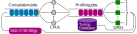
\includegraphics[width=.6\columnwidth]{extra/autotuner.pdf}
  \caption{Multithreaded autotuning pipeline for kernels}
  \label{fig:comp_work_queue}
\end{figure}

% Uncomment if have space
%
%The autotuner varies multiple options, among others it tunes:
%\begin{itemize}
%\item grid and block sizes, loop \emph{tiling} parameters (powers of 2 and
%integer ceil divisors of the problem size);
%\footnote{In our experience, for latency-bound kernels, it is often preferable
%to avoid launching an extra block for problem sizes close to a power of $2$
%(e.g., $130$) by using a slightly larger block size.}
%\item the bound on the number of iterations to \emph{unroll} (powers of 2 up to
%$256$);
%\item discrete choices on loop fusion, schedule shapes, promotion to shared
%memory and registers.
%\end{itemize}

Each generated version is ``warmed up'' by a few
executions before being profiled.  Without any performance guarantees,
autotuning needs to quickly prune poor candidates.  Because CUDA
kernels cannot be stopped once launched,
we rely on the following pruning heuristics to decrease the
autotuning time by an order of magnitude. (1) Parameter specialization
allows the exact number of active threads and blocks to be computed beforehand.
Kernels with fewer threads than some configurable threshold (e.g., $256$) are
not launched. (2) If during the first run, a kernel is more
than $100\times$ slower than the best version so far, or it is $5\times$ slower
after warmup, it is pruned immediately.

While autotuning time may become significant, compilation and
autotuning time is not a fundamental limit to TC's applicability.  In
training scenarios, a significant amount of time is spent on computing
the same kernel repeatedly over different data during the (stochastic)
gradient descent.  In inference scenarios, the network is optimized
ahead of time. As a result, although TC operates as a JIT compiler, it
only marginally hits the typical compilation/run-time trade-offs of
JIT compilers. Autotuning time may become an issue in specific
training scenarios where hyper-parameters would need to be frequently
updated, but in such a case one may leverage TC's intrinsic handling
of dynamic shapes and generate a single version of each operator or
fused operators to handle all hyper-parameter configurations.

%%Uncomment if have space
%In the future we plan to drive this pruning and, more generally, the search
%with a model but for the time being, we deem the user experience of our tuning
%flow satisfactory.

\section{Integration with ML Frameworks}
TC is designed to optimize individual layers or small subgraphs of an ML model.
Considering the entire model is not only computationally expensive, but often
leads to most transformations being hindered by a large number of data
dependences. Furthermore, ML frameworks perform work distribution and placement
at the model level, treating a layer as a unit of work; extremely large layers
could interfere with the framework operation.

Unlike XLA or Glow, TC supports completely custom layers.  In TC,
\emph{layer fusion} is merely pasting the code that constitutes the
layers into a single function, or inlining TC functions at the AST
level. Unlike Halide and TVM, the polyhedral backbone of TC includes
instance-wise dependence analysis, capturing dependences and tensor
access relations at the level of individual loop iterations and tensor
elements. This allows TC to fuse operations without introducing
redundant computation, and to combine fusion with enabling
transformations such as shifting (for convolutions) or
scaling (for pooling layers). TC's polyhedral representation also
enables it to automatically infer sizes, and to discover parallelism and
locality-parallelism trade-offs beyond a predefined collection of
map/reduce/scan combinators.

Let us now describe the transparent integration into a ML framework,
from a user perspective.  Until now, such levels of integration had
only been demonstrated on operator graph compilers such as XLA \cite{XLA}
and Glow \cite{Glow}, starting from a lower level of abstraction than TC,
and missing the genericity and high reusability of a polyhedral
framework as well as feedback-directed autotuning.

We opted for an ``in process'' implementation, streamlining the interaction
with computation graph engines and ML applications built on top of them, a
unique feature for a fully-automated scheduling and mapping flow.
TC is integrated into any ML framework as follows.  We provide a thin API that
translates the specific tensor object model to our own, see
\figref{integration}. Operator definitions are overridden to generate TC rather
than the framework's backend implementation, as well as provide users the
ability to write their own TC.  A single TC may correspond to a DAG of
operators in the ML framework.
The tensor comprehensions are then JIT-compiled as shown in \figref{flow}.
DAG partitioning, matching and rewriting (like, e.g.,
TensorRT~\cite{TensorRT}) is currently not part of the flow, although
this would make an interesting future combination,
with feedback from the compiler.

\begin{figure}[h!tb]
\vskip-1em
\begin{minipage}{.56\textwidth}
\begin{cpplisting}
string tc = R"TC(some_tc_for_conv)TC";
auto I = makeATenTensor<CudaBackend>({N, C, H, W});
auto W = makeATenTensor<CudaBackend>({F, C, KH, KW});
ATenAutotuner<CudaBackend> tuner(tc);
auto best = tuner.tune("conv", {I, W});
auto pExecutor =
    compile<CudaBackend>(tc, "conv", {I, W}, best[0]);
auto out = prepareOutputs(tc, "conv", {I, W});
auto times = profile(*pExecutor, {I, W}, outs);
\end{cpplisting}
\end{minipage}
\begin{minipage}{.42\textwidth}
\begin{pylisting}
import torch
import tensor_comprehensions as tc
tcdef = """...some_tc_for_conv..."""
T_I = torch.randn(N, C, H, W).cuda()
T_W = torch.randn(F, C, KH, KW).cuda()
# register the TC string
conv = tc.define(tcdef, name="conv")
# autotune the kernel
best = conv.autotune(T_I, T_W)
# run with best option and cache the binary
T_O = conv(T_I, T_W, options=best)
\end{pylisting}
\end{minipage}
\vskip-1em
\caption{Example of embedded usage in C++/ATen (top) and PyTorch (bottom)}
\label{fig:integration}
\end{figure}

\section{Performance Results}

We evaluate our framework on 2 systems:
(1) Nvidia Pascal nodes with 2 socket, 14 core Intel(R) Xeon(R) CPU E5-2680
v4 @ 2.40GHz, with 2 Quadro P100-12GB; and
(2) Nvidia Volta nodes with 2 socket, 20 core Intel(R) Xeon(R) CPU E5-2698
v4 @ 2.20GHz, with 8 Tesla V100-SXM2-16GB.
Both systems use CUDA 9.0 and cuDNN 7.0.
% which are the most recent versions available on our HPC cluster.

We report results for 9 TC functions ranging from a simple matrix
multiplication kernel to a full WaveNet cell~\cite{WaveNet}. The
individual benchmarks are described below: \figref{benchmarks} and
\figref{wavenet} show the complete source code. The matrix
multiplication and convolution kernels were selected for their
dominance of the training and inference time of the most classical
networks \cite{Awan:2017:IPC:3146347.3146356,ResNext}. The other
kernels bring interesting computation patterns to enable
expressiveness and performance comparisons in more diverse network
architectures.

These results are all based on TC commit
\texttt{2e1a0dc54850} % 163fc59ac2f8bc51e9decf531b6c
available at \\
\url{https://github.com/nicolasvasilache/TensorComprehensions}.

Running the autotuner for 25 generations of 100 candidates, the
(parallel) autotuning process takes up to 1h on the longest running
kernels, and 6h in total.\footnote{Classical strategies exist to
  accelerate autotuning, such as predictive modeling and search space
  pruning \cite{Agakov:2006:UML:1121992.1122412}, but this was not the
  focus of this paper.}

\begin{figure}[h!tb]
\begin{tclisting_small}
def tmm(float(M,K) A, float(N,K) B) -> (C) { C(m,n) +=! A(m,r_k) * B(n,r_k) }
def tbmm(float(B,N,M) X, float(B,K,M) Y) -> (Z) { Z(b,n,k) +=! X(b,n,r_m) * Y(b,k,r_m) }

def 1LUT(float(E1,D) LUT1, int(B,L1) I1) -> (O1) { O1(i,j) +=! LUT1(I1(i,r_k),j) }
def 2LUT(float(E1,D) LUT1, int(B,L1) I1, float(E1,D) LUT1, int(B,L1) I1) -> (O1, O2) {
  O1(i,j) +=! LUT1(I1(i,r_k),j)
  O2(i,j) +=! LUT2(I2(i,r_k),j)
}

def MLP3(float(B,M) I, float(O,N) W2, float(O) B2, float(P,O) W3, float(P) B3, float(Q,P) W4,
	 float(Q) B4) -> (O1,O2,O3,O4) {
  O2(b,o)  = B2(o)
  O2(b,o) += O1(b,r_n) * W2(o,r_n)
  O2(b,o)  = fmaxf(O2(b,o), 0)
  O3(b,p)  = B3(p)
  O3(b,p) += O2(b,r_o) * W3(p,r_o)
  O3(b,p)  = fmaxf(O3(b,p), 0)
  O4(b,q)  = B4(q)
  O4(b,q) += O3(b,r_p) * W4(q,r_p)
  O4(b,q)  = fmaxf(O4(b,q), 0)
}

def kronecker3(float(D0,N0) W0, float(D1,N1) W1, float(D2,N2) W2, float(M,N0,N1,N2) X) -> (Y,XW1,XW2) {
  XW2(m,n0,n1,d2) +=!   X(m,n0,n1,r_n2) * W2(d2,r_n2)
  XW1(m,n0,d1,d2) +=! XW2(m,n0,r_n1,d2) * W1(d1,r_n1)
    Y(m,d0,d1,d2) +=! XW1(m,r_n0,d1,d2) * W0(d0,r_n0)
}

def group_convolution(float(N,G,C,H,W) I, float(G,F,C,KH,KW) W1, float(M) B) -> (O) {
  O(n,g,o,h,w)  = O(n,g,o,h,w) + B(m)
  O(n,g,o,h,w) += I(n,g,r_i, h + r_kh, w + r_kw) * W1(g,o,r_i,r_kh,r_kw)
}

def moments2_2d_1D(float(N,K) I) -> (mean,var) {
# var = E(x^2) - mean^2
  mean(n) +=! I(n,r_k)
  var(n)  +=! I(n,r_k) * I(n,r_k)
  mean(n)  =  mean(n) / K
   var(n)  =  var(n) / K - mean(n) * mean(n)
}

def group_normalization(float(N,G,D,H,W) I, float(G,D) gamma, float(G,D) beta,
			float(N,G) mean, float(N,G) var) -> (O,mean,var) {
  O(n,g,d,h,w) = gamma(g,d) * (I(n,g,d,h,w) - mean(n,g))
	       * rsqrt(var(n,g) - mean(n,g) * mean(n,g) + 1e-5) + beta(g,d)
}

def group_normalization_single_kernel(float(N,G,D,H,W) I, float(G,D) gamma,
				      float(G,D) beta) -> (O,mean,var) {
  mean(n,g) +=! I(n,g,r_d,r_h,r_w)
  var(n,g)  +=! I(n,g,r_d,r_h,r_w) * I(n,g,r_d,r_h,r_w)
  O(n,g,d,h,w) = gamma(g,d) * (I(n,g,d,h,w) - mean(n,g) / (D * H * W)) * rsqrt(var(n,g)/(D * H * W)
                 - mean(n,g)/(D * H * W) * mean(n,g)/(D * H * W) + 1e-5) + beta(g,d)
}
\end{tclisting_small}
  \vskip-1em
\caption{TC Benchmarks used in the experiments.  Evaluated sizes are available in Table~\ref{tbl:absolute}}
\label{fig:benchmarks}
\end{figure}

\begin{figure}[h!tb]
\begin{tclisting_small}
def wavenet1(float(B, RESIDUAL_C, RECEPTIVE_FIELD) Data,
             float(DILATION_C, RESIDUAL_C, 2) FilterWeight, float(DILATION_C) FilterBias,
             float(DILATION_C, RESIDUAL_C, 2) GateWeight, float(DILATION_C) GateBias,
             float(RESIDUAL_C, DILATION_C) ResWeight, float(RESIDUAL_C) ResBias,
             float(SKIP_C, DILATION_C) SkipWeight, float(SKIP_C) SkipBias,
             float(DILATION_FACTOR) Dilation)
    -> (FilterOut, GateOut, NonLin, Res, Skip) {
  FilterOut(b, dilation_c, rf)  = FilterBias(dilation_c)
    where b in 0:B, dilation_c in 0:DILATION_C, rf in 0:RECEPTIVE_FIELD
  FilterOut(b, dilation_c, rf) += Data(b, r_residual_c, rf)
      * FilterWeight(dilation_c, r_residual_c, 1) + ((rf - DILATION_FACTOR >= 0)
        ? Data(b, r_residual_c, rf - DILATION_FACTOR) * FilterWeight(dilation_c, r_residual_c, 0)
        : float(0))
      where rf in 0:RECEPTIVE_FIELD

  GateOut(b, dilation_c, rf)  = GateBias(dilation_c)
    where b in 0:B, dilation_c in 0:DILATION_C, rf in 0:RECEPTIVE_FIELD
  GateOut(b, dilation_c, rf) += Data(b, r_residual_c, rf)
      * GateWeight(dilation_c, r_residual_c, 1) + ((rf - DILATION_FACTOR >= 0)
        ? Data(b, r_residual_c, rf - DILATION_FACTOR) * GateWeight(dilation_c, r_residual_c, 0)
        : float(0))
      where rf in 0:RECEPTIVE_FIELD

  NonLin(b, dilation_c, rf)  = tanh(FilterOut(b, dilation_c, rf))
    where rf in 0:RECEPTIVE_FIELD
  NonLin(b, dilation_c, rf) *= 1 / (1 + exp(-GateOut(b, dilation_c, rf)))
    where rf in 0:RECEPTIVE_FIELD

  Res(b, residual_c, rf)  = Data(b, residual_c, rf) + ResBias(residual_c)
  Res(b, residual_c, rf) += NonLin(b, r_dilation_c, rf) * ResWeight(residual_c, r_dilation_c)

  Skip(b, skip, rf) +=! NonLin(b, r_dilation_c, rf) * SkipWeight(skip, r_dilation_c)
    where rf in 0:RECEPTIVE_FIELD
  Skip(b, skip, rf)  =  Skip(b, skip, rf) + SkipBias(skip)
    where rf in 0:RECEPTIVE_FIELD
}
\end{tclisting_small}
  \vskip-1em
\caption{Source of one full WaveNet cell}
\label{fig:wavenet}
\end{figure}

\begin{figure}[h!tb]
  \center  
  \includegraphics[width=8cm]{extra/tc_p100_caffe2_p100}
  \vskip-1.5em
  \caption{Speedup of TC-generated kernels over Caffe2 hand-tuned kernels on Quadro P100-12GB}
  \label{fig:pairwise_p100}

  \center
  \includegraphics[width=8cm]{extra/tc_v100_caffe2_v100}
  \vskip-1.5em
  \caption{Speedup of TC-generated kernels over Caffe2 hand-tuned kernels on Tesla V100-SXM2-16GB}
  \label{fig:pairwise_v100}

  \center
  \includegraphics[width=9cm,keepaspectratio]{extra/v100_all.pdf}
  \vskip-1.5em
  \caption{\label{fig:perf}Relative performance: baseline is Caffe2
    performance on a P100 GPU}
\end{figure}

The relative performance of kernels automatically generated with TC compared to
Caffe2
is shown in \figref{pairwise_p100} and \figref{pairwise_v100}.%
\footnote{We compile Caffe2 and PyTorch from source
  (commit \texttt{6223bfdb1d32}) and integrate it in the TC testing flow
  for proper benchmarking.}
%Caffe2 is one of the fastest ML
%frameworks available and has enjoyed a close collaboration between Facebook
%and Nvidia with more than 100 contributors.
%Caffe2 efficiently wraps cuBLAS, CUB and cuDNN where relevant and provides its
%own CUDA implementations when libraries fall short.
Caffe2 provides a very strong baseline by wrapping tuned implementations, which
originate from either hand-tuned libraries or other high-performance code
generators.\footnote{A recent unification effort~\cite{F82018} made Caffe2 the
backend for PyTorch~1.0.}
\emph{We chose to compare against Caffe2 rather than against other optimization
flows due to expressivity and automation limitations}: XLA or Glow do not
support custom layers, and Halide or TVM lack range inference and automatic
parallelism discovery, which significantly complicates the expression of new
layers such as KRU and WaveNet.  The common set of comparable layers would be
limited to matrix multiplications and convolutions, while one of the main
contributions of TC is to enable exploration of new unconventional layers
\emph{before super-optimized implementations are available}.

In addition, \figref{perf} brings together the performance of TC-compiled kernels on both GPU systems, normalized to Caffe2 on P100.
This consolidated graph conveys 3 classes of information in a
common context: (1) speedup of Caffe2 V100 over Caffe2 P100 to illustrate the
out-of-the-box benefits (or lack thereof) of a faster GPU; (2) speedup of TC over Caffe2 on
P100 (main comparison); and (3) speedup of TC V100 over Caffe2
P100. The last choice may seem surprising, but presented in the context
of the other two,
allows for relative comparisons: the height of the Caffe2 V100 and TC
V100 captures the raw speedups of TC on V100.
% Alex removed "better mental model" here; until further advances, we cannot
% control the mental model of the reader...
\emph{We aim at compactly illustrating that TC provides a path to
  performance portability, improving on state of the
  art frameworks and library primitives}.

\tblref{absolute} provides absolute runtime running TC and Caffe2; all values are reported in $\mu s$.

\begin{table*}[h!tb]
{\footnotesize% 1LUT TC     Caffe2
\renewcommand{\arraystretch}{.5}
\begin{tabular}{llrrrrrr}
\toprule
	      &  &  & {\textbf{Pascal}} &  &  & {\textbf{Volta}} & \\
\textbf{1LUT} &  & p0 & p50 & p90 & p0 & p50 & p90\\
\midrule
\multirow{2}{*}{$B = 128, D = 64, E1 = 10^7, L1 = 50$}
  & TC     & 13 & 14 & 14 & 15 & 16 & 17\\
  & Caffe2 & 85 & 91 & 95 & 56 & 58 & 63\\

% 2LUT TC     Caffe2
\toprule
\textbf{2LUT} &  & p0 & p50 & p90 & p0 & p50 & p90\\
\midrule
\multirow{2}{*}{
$B = 128, D = 64, E1, E2 = 10^7, L1, L2 = 50$}
  & TC     & 52 & 54 & 57 & 35 & 35 & 37\\
  & Caffe2 & 132 & 136 & 144 & 115 & 117 & 124\\

% MLP1 TC     Caffe2
\toprule
\textbf{MLP1} &  & p0 & p50 & p90 & p0 & p50 & p90\\
\midrule
\multirow{2}{*}{$B = 128, M = 2000, N = 128$}
  & TC     & 68 & 69 & 71 & 57 & 58 & 59\\
  & Caffe2 & 87 & 89 & 91 & 116 & 118 & 123\\

% MLP3 TC     Caffe2
\toprule
\textbf{MLP3} &  & p0 & p50 & p90 & p0 & p50 & p90\\
\midrule
\multirow{2}{*}{$B = 128, N = 128, O = 64, P = 32, Q = 2$}
  & TC     & 18 & 19 & 19 & 20 & 20 & 21\\
  & Caffe2 & 157 & 159 & 169 & 144 & 146 & 164\\

% BatchMatMul TC     Caffe2
\toprule
\textbf{tbmm} &  & p0 & p50 & p90 & p0 & p50 & p90\\
\midrule
\multirow{2}{*}{$B = 500, K = 26, M = 72, N = 26$}
  & TC     & 52 & 53 & 54 & 42 & 43 & 43\\
  & Caffe2 & 94 & 102 & 103 & 76 & 77 & 78\\

% GroupConvolution TC     Caffe2
\toprule
\textbf{Group Convolution} &  & p0 & p50 & p90 & p0 & p50 & p90\\
\midrule
$C, F = 4, G, N = 32, H = 56, \textit{KH}, \textit{KW} = 3,$ & TC      & 696 & 701 & 704 & 435 & 440 & 443\\
$W = 56$                                                     & Caffe2  & 1590 & 1609 & 1621 & 879 & 888 & 896\\
\midrule
$C, F = 8, G, N = 32, H = 28, \textit{KH}, \textit{KW} = 3,$ & TC      & 574 & 576 & 578 & 269 & 270 & 272\\
$W = 28$                                                     & Caffe2  & 640 & 653 & 692 & 613 & 650 & 660\\
\midrule
$C, F = 16, G, N = 32, H = 14, \textit{KH}, \textit{KW} = 3,$ & TC     & 265 & 272 & 276 & 274 & 284 & 287\\
$W = 14$                                                      & Caffe2 & 440 & 474 & 510 & 377 & 383 & 397\\
\midrule
$C, F = 32, G, N = 32, H = 7, \textit{KH}, \textit{KW} = 3,$ & TC       & 463 & 481 & 491 & 259 & 260 & 264\\
$W = 7$                                                      & Caffe2   & 456 & 461 & 469 & 367 & 388 & 394\\

% GroupNormalization TC     Caffe2
\toprule
\textbf{Group Normalization} &  & p0 & p50 & p90 & p0 & p50 & p90\\
\midrule
\multirow{2}{*}{$C = 512, G = 32, H = 12, N = 4, W = 12$}
  & TC      & 22 & 23 & 24 & 32 & 33 & 35\\
  & Caffe2  & 37 & 38 & 40 & 33 & 34 & 35\\
\midrule
\multirow{2}{*}{$C = 512, G = 32, H = 48, N = 32, W = 48$}
  & TC     & 1285 & 1290 & 1294 & 593 & 597 & 601\\
  & Caffe2 & 1814 & 1819 & 1823 & 865 & 869 & 871\\

% TransposedMatMul TC     Caffe2
\toprule
\textbf{tmm} &  & p0 & p50 & p90 & p0 & p50 & p90\\
\midrule
\multirow{2}{*}{$K = 32, M = 128, N = 256$}
  & TC     & 15 & 15 & 15 & 15 & 16 & 17\\
  & Caffe2 & 18 & 19 & 20 & 31 & 31 & 32\\
\midrule
\multirow{2}{*}{$K = 1024, M = 128, N = 1024$}
  & TC     & 318 & 334 & 344 & 181 & 189 & 192\\
  & Caffe2 & 55 & 58 & 64 & 89 & 90 & 91\\
\midrule
\multirow{2}{*}{$K = 4096, M = 128, N = 16384$}
  & TC     & 17168 & 17209 & 17270 & 7937 & 8004 & 8096\\
  & Caffe2 & 2254 & 2388 & 2590 & 1360 & 1378 & 1419\\
\bottomrule
\end{tabular}

}
\caption{Absolute run time in $\mu s$}
\label{tbl:absolute}
\vskip-.5cm
\end{table*}

\paragraph{TMM: Transposed Matrix-Multiplication}
On matrix multiplications of shapes and sizes relevant to deep learning
workloads (i.e., small $128\times 32\times 256$,
medium $128\times 1024\times 1024$ and large $128\times 4096\times 16384$), TC
does not perform competitively, except in the low-latency small case. This is
due to: (1) the lack of a target-specific register blocking optimization, making
kernels bound by shared memory bandwidth which is an order of magnitude slower
than register bandwidth; (2) the lack of target-specific, basic-block level optimizations including careful register allocation and instruction scheduling. Matrix multiplication is the most tuned
computation kernel in history: the missing optimizations are all well known, and
may be found in use cases and open source implementations such like
CUTLASS~\cite{CUTLASS}. Alternatively, polyhedral compilation has been shown to match or outperform cuBLAS, provided sufficient target- and operator-specific information has been captured in the optimization heuristic and code generator \cite{Elango:2018:DDL:3211346.3211354}. While our scientific focus was on covering a wide range of layers with TC, a production release would need to embed such operator-specific strategies as well. One strategy would be to follow the classification and heuristic steering of Kong et al.\ \cite{KongVocabulary}. Also, TC does not replace all layers: it only acts as a custom operation in a graph; one may use TC concurrently with numerical libraries as well as custom implementations provided through TVM.

\paragraph{Group Convolution}
Group convolution is expressible with 2 lines of TC. We report comparisons for
sizes relevant to the ResNext model~\cite{ResNext}. Despite not
using either register optimizations, Fourier or Winograd domain convolutions,
TC produces faster kernels than the cuDNN ones, with running times between
$250\mu$s and $750\mu$s. To check how TC fares w.r.t.\ recent advances in optimizing group convolutions, we performed an additional comparison with the
PyTorch nightly package \ic{py36_cuda9.0.176_cudnn7.1.2_1} with
\ic{torch.backends.cudnn.benchmark=True}. TC speedups range
from $-2\%$ to $8\times$. We also observe
PyTorch performance on V100 to be worse than on P100 while TC achieves
performance portability.

\paragraph{Group Normalization}
Group Normalization was recently proposed as a way to overcome limitations of
Batch Normalization at smaller batch sizes and increase parallelism
\cite{GroupNorm}. In TC,
group normalization is a 5-line function. TC performance is
roughly $30\%$ better than the hand-tuned Caffe2 implementation. Whereas Caffe2
uses 4 \emph{handwritten} CUDA kernels, we chose to write the TC version as two
separately compiled TC functions for better reuse and overall performance.
We also experimented with writing a single fused TC but performance degraded.
This is mostly due to kernels requiring substantially different grid
configurations, which makes their fusion unprofitable.  A larger, graph-level
compiler that decides on TC function granularity, informed by the TC mapper and
the autotuner is necessary to automate this decision process, but is left for
future work.

\paragraph{Production Model}
The kernels \ic{1LUT}, \ic{2LUT}, \ic{MLP1} and \ic{MLP3} are the
backbone of a low-latency production model used at scale in a large company
and correspond to (1) reductions over a large lookup table embedding (10M
rows); (2) fused reduction over 2 large lookup table embeddings (10M rows);
(3) small size Multi-Layer Perceptron (fully-connected, bias, ReLU); and
(4) very small size, 3 consecutive Multi-Layer Perceptrons.
Despite LUT sizes, this model is essentially latency-bound.
Existing libraries are often not tuned for low-latency regimes and tend to
perform poorly.

On these examples, the need for reuse and instruction-level
parallelism is dwarfed by the need to quickly load data from the memory
into registers. TC is able to adapt to the problem size, leveraging
reduction parallelism to hide memory latency.
% AC: removed, not implemented, it was only available in PPCG-based c2isl
% and promoting indirectly referenced arrays to shared memory
This results in large speedups over Caffe2 with cuBLAS 9.0.

\paragraph{Transposed Batch MatMul}
This kernel is meant as a case study to characterize performance benefits and losses in the current flow, compared with reference libraries.
For the sizes relevant to Factorization Machines~\cite{Rendle2010}, ($500
\times 26 \times 72 \times 26$), Nvidia Profiler reports
the TC autotuned
kernel taking 56$\mu$s on the Nvidia Quadro P6000 GPU (Pascal) while both Pytorch and Caffe2 resort to the specialized cuBLAS function
\texttt{maxwell\_sgemm\_128x64\_nn} that takes 87$\mu$s.
Beyond architecture mismatch indicated in the function name, a detailed
performance comparison demonstrates that TC executes 500 blocks of $26
\times 13 = 338$ threads, compared to 500 blocks of $128$ threads for cuBLAS,
reaching $81.8\%$ occupancy instead of $23.6\%$.
Additionally,
the cuBLAS kernel shows a large number of predicated-off instructions
due to the block size not matching the problem size.
Occupancy is limited by the number of registers in both
cases (11264 vs.\ 15360), but the TC version can be distributed over~5 blocks instead of~4.\footnote{Mapping to blocks of $32 \times 13$ threads to obtain full warps
results in 60$\mu$s execution time and only 4 blocks due to the higher number of
registers per block.}
TC promotes all tensors to shared memory, saturating its bandwidth, whereas arithmetic instructions are the performance limiter for cuBLAS.
Given the large occupancy metric, performance can be further increased by promoting one tensor to
registers instead, trading off lower occupancy for reduced pressure on memory bandwidth.

\paragraph{Kronecker Recurrent Units}
These have been recently proposed as a solution to drastically reduce
model sizes by replacing the weights matrix of a linear layer by a
Kronecker product of much smaller matrices~\cite{KRU17}.  In TC, a
Kronecker product of 3 matrices is easily written as shown in the
\texttt{kronecker3} function in \figref{benchmarks}.
The following table shows
the running time in $\mu s$---or out of memory (OOM)---of a large
matrix multiplication in Caffe2 and the equivalent Kronecker product
of 3 matrices.  Note that \emph{the performance difference mostly
  comes form a using a different algorithm}.  While no specialized GPU
library primitives exist for Kronecker recurrent units, TC's automatic
flow enabled rapid exploration and reaching unprecedented levels of
performance, as shown in \tblref{kruperf}.
Clearly, this benchmark deserves a deeper discussion of the space of
possible TC derivations, including memory/computation/parallelism trade-offs
falling outside the scope of this paper.
The \texttt{kronecker3} function is one such possible implementations that
performed well for the three selected matrix shapes;
it avoids redundant computation at the expense of storage
(two tensors for intermediate computations).

\paragraph{WaveNet}
WaveNet~\cite{WaveNet} is a popular model that enables generation of realistic sounding
voices as highlighted at Google I/O 2018. We encoded a full WaveNet cell
using a single TC function and compared our generated kernel
with a WaveNet layer from PyTorch. This experiment uses a batch
size of $1$, residual and dilation channels of $32$, and $256$ skip
channels.
With TC, we observe performance improvements up to $4\times$ on Volta, as shown on \tblref{wavenetperf}.

\begin{table*}[h!tb]
\begin{center}
\renewcommand{\arraystretch}{.5}
{\footnotesize
\begin{tabular}{llrrrrrr}
  \toprule
\textbf{Algorithmic exploration} & &  & \textbf{Pascal} &  &  & \textbf{Volta} & \\
\textbf{of Kronecker Recurrent Units} & & p0 & p50 & p90 & p0 & p50 & p90\\
  \midrule
& TC Kronecker                              & 272 & 280 & 285 & 200 & 206 & 212\\
$256\times 16^3\times 32^3$ & Caffe2 MatMul & 7714 & 8158 & 8216 & 4946 & 5065 & 5466\\
  \midrule
& TC Kronecker                              & 1334 & 1349 & 1365 & 998 & 1004 & 1011\\
$256\times 16^3\times 64^3$ & Caffe2 MatMul & 64499 & 64765 & 65659 & 38280 & 39307 & 39327\\
  \midrule
& TC Kronecker                                         & 4408 & 4447 & 4472 & 4794 & 4815 & 5106\\
$256\times 16^3\times 64 \times 128^2$ & Caffe2 MatMul & OOM & OOM & OOM & OOM & OOM & OOM\\

% WaveNet autotuned
  \toprule
\textbf{WaveNet Cell}& & p0 & p50 & p90 & p0 & p50 & p90\\
  \midrule
$\mathrm{receptive~field}=4K,~\mathrm{dilation}=1$ & TC & 457 & 466 & 477 & 253 & 255 & 257\\
$\mathrm{receptive~field}=4K,~\mathrm{dilation}=1$ & PyTorch & 549 & 576 & 790 & 563 & 571 & 594\\
  \midrule
$\mathrm{receptive~field}=4K,~\mathrm{dilation}=32$ & TC & 353 & 365 & 375 & 138 & 139 & 140\\
$\mathrm{receptive~field}=4K,~\mathrm{dilation}=32$ & PyTorch & 551 & 574 & 630 & 562 & 569 & 585\\
  \bottomrule
\end{tabular}
}
\end{center}
\caption{Algorithmic exploration of Kronecker Recurrent Units and optimization of a WaveNet cell}
\label{tbl:kruperf}
\label{tbl:wavenetperf}
\vskip-.5cm
\end{table*}

\section{Related Work}

Despite decades of progress in optimizing and parallelizing
compilation, programmers of computationally intensive applications
complain about the poor performance of optimizing compilers, often
missing the machine peak by orders of magnitude. Among
the reasons for this state of the affairs, one may cite the complexity
and dynamic behavior of modern processors, domain knowledge required
to prove optimizations' validity or profitability being unavailable to
the compiler, program transformations whose profitability is difficult
to assess, and the intrinsic difficulty of composing complex
transformations, particularly in the case of computationally intensive
loop nests \cite{URUK,Clay}.

Several contributions have successfully addressed this issue, not by improving
a general-purpose compiler, but through the design of
application-specific program generators, a.k.a.\ active libraries
\cite{VG98}. Such generators often rely on feedback-directed
optimization to select the best generation schema \cite{Smi00}, as
popularized by ATLAS \cite{ATLAS} for dense matrix operations (and more
recently BTO \cite{BTO09}) and FFTW
\cite{FFTW} for the fast Fourier transform.
Most of these generators use transformations previously proposed for
traditional compilers, which fail to apply them for the aforementioned
reasons. The SPIRAL project
\cite{SPIRAL} made a quantum leap over these active libraries, operating on a
domain-specific language (DSL) of digital signal processing formulas.
Compilers for DSLs typically rely on domain-specific constructs to capture the
intrinsic parallelism and locality of the application.  Using such an
approach, DSL compilers such as Halide~\cite{Halide} for image processing show
impressive results. Its inputs are images defined on an infinite range while
TC sets a fixed size for each dimension using range inference. This is better
suited to ML applications, dominated by fixed size tensors with
higher temporal locality than 2D-images; it is also less verbose in the case of
reductions and does not carry the syntactic burden of anticipating the declaration of stage
names and free variables (Halide needs this as a C++ embedded DSL).
OoLaLa~\cite{OoLaLa} takes a similar approach for linear algebra, and
TACO~\cite{Taco} and Simit~\cite{Simit} use a similar notation as TC but
generate sparse matrix code for numerical solvers.

Following this trend in the context of deep neural networks, we not only
design yet another DSL and compiler but propose a more generic code generation
and optimization framework bringing together decades of research in loop nest
optimization and parallelization for high-performance computing. We also
design the domain language to cover a variety of existing and emerging machine
learning models.
Our framework automates a combination of affine transformations involving
hierarchical tiling, mapping, shifting, fusion, distribution, interchange, on
either parametric or fully instantiated problems, that are not accessible to
Halide \cite{Halide,Mullapudi2016HalideAutoscheduler}, Latte \cite{Latte} or
XLA's \cite{XLA} representations of tensor operations.

% \aanote{Some too-verbose thoughts on the Halide comparison: The algorithm
% specification is syntactically identical to the Halide specification of the
% same thing! You could copy-paste it. Reviewers may notice. Bounds, however,
% are treated in a fundamentally different manner more suited to tensor
% computations. Just like Halide, bounds are inferred, but Halide treats
% pipeline stages as functions defined over an infinite integer domain, and
% infers bounds based on what regions are used (demand-driven bounds
% inference), stages in one of these pipelines have algorithmically meaningful
% sizes, and bounds are supply-driven. They're inferred based on the size of
% the *input*. One concrete advantage of this over Halide is that bounds on
% reduction dimensions can be inferred. In Halide these must be specified
% manually using an "RDom". Halide is also cluttered with the need to
% predeclare the stage names and free variables to make the code legal C++.
% Not sure how to turn this into paper text. The thing I would emphasize is
% the syntactic equivalent and the backwards vs forwards difference in bounds
% inference.}
% \acnote{I suggest we insert a very language-specific comparison in this
% paragraph, more discriminating than the above text, and explicitly defer the
% rest of the comparison to the related work section. Zack, do you see a way
% to refine the comparison of the language designs that could better highlight
% the technical advantages of TC? It does not have to be innovative in all
% dimensions of course, but one key advantage of TC motivating the design of a
% new language should be found for each related language, as TC is presented
% as one of the top level contributions. Safety, performance, conciseness,
% domain-suitedness, etc., anything.}

% \ntvnote{Add references to FLAME}\acnote{Not needed, no GPU target beyond a
% couple of preliminary research papers and experiments}

The polyhedral framework is a powerful abstraction for the analysis
and transformation of loop nests, and a number of tools and libraries
have been developed to realize its benefits
\cite{feautrier92multi,Bondhugula2008Pluto,PPCG2013,Bondhugula2016Pluto+,Zinenko2018Spatial},
including production compilers such as GCC (Graphite) and LLVM
(Polly).  Polyhedral techniques have also been tailored for
domain-specific purposes. State of the art examples include the
PolyMage~\cite{Polymage} DSL for image processing pipelines and the
PENCIL approach to the construction of parallelizing and compilers for
DSLs~\cite{Baghdadi2015Pencil,VOBLA}. PolyMage is a clear illustration
of the benefits of operating at a high level of abstraction, closer to
the mathematics of the domain of interest: while GCC/Graphite and
LLVM/Polly struggle to recover affine control and flow from low-level
code, PolyMage natively captures patterns amenable to domain-specific
optimization, such as stencil-specific overlapped tiling with or
without recomputation, and cache-conscious fusion and tiling
heuristics; it also offers a more productive programming experience
for end users.  Interestingly, some techniques derived from PolyMage
crossed out of polyhedral representations into Halide's automatic
scheduler~\cite{Mullapudi2016HalideAutoscheduler}.  Back to deep
learning frameworks, TVM extends Halide with recurrent (parallel scan)
operators, support for ML accelerators, and tight integration with ML
frameworks \cite{TVM}. It also provides autotuning
capabilities \cite{autotvm} and shares
several engineering goals of TC, such as transparent ML framework
integration.  Much like PolyMage, TC implements optimizations well
suited to the long distance, non-uniform reuse patterns of deep
learning models; these heuristics are not available in general-purpose
compilers such as LLVM/Polly, Pluto or PPCG, or semi-automatic frameworks
such as Halide and TVM.

None of the aforementioned frameworks offer the
complete transparency of TC's end-to-end compilation flow.
TVM involves some level of manual intervention and/or feedback-directed
optimization even for producing the most baseline GPU implementation,
and it guarantees functional correctness for a
subset of the scheduling primitives and tensor operations: e.g.,
convolutions can only be fused at the expense of introducing redundant
computations, or involving lower level transformations that cannot be
verified at compilation time. In addition, the balance between
analytical objective functions (profitability heuristics) and
feedback-directed autotuning is completely different: Halide and TVM
auto-schedulers expose all scheduling decisions to the autotuner and
infer most performance-related information from execution profiles,
while TC's polyhedral flow reduces the autotuning space to a narrow
set of optimization options and tile sizes.

% \ntvnote{cite Loopy when metaprogramming or matching gets in}

% \acnote{Removed Delite, cited in the introduction (indirectly) and not directly relevant.}

% Delite \cite{chafi_domain-specific_2011} is a generic
% framework for building DSL compilers.
% Delite uses Lightweight Modular Staging (LMS) \cite{lms_staging_10}, a compiler framework designed for embedding DSLs into Scala.
% Delite relies on information from a DSL to decide whether a loop is
% parallel but has no facilities for advanced loop nest transformations and automatic acceleration on a GPU.

% \acnote{Discuss stratego/matching/rewrite systems after we converge on the annotation and pattern matching section}

TC also shares several motivations with Latte \cite{Latte} and PlaidML
\cite{PlaidML}, including a high level domain-specific language and an
end-to-end flow.  TC provides elementwise access that is just as
expressive when implementing custom layers, but unlike Latte it is
more concise thanks to type and shape inference, safer regarding
static bound checking and graph connectivity, and more flexible by
decoupling indexing from representation and layout choices.
In addition, our framework implements more complex
scheduling and mapping transformations than both Latte and PlaidML,
some of which are essential to GPU targets with partitioned memory
architectures. Unlike Latte, it is also designed as a JIT compilation
library for seamless integration with deep learning frameworks. Unlike
PlaidML, it is not limited to high level patterns and rewrite rules,
but captures complex affine transformations resulting from analytical
modeling and autotuning. As a consequence, the TC compilation process
takes generally more time than PlaidML, a price to pay for the ability
to implement a wider range of optimizations.

Like TC, XLA \cite{XLA} provides automatic shape and size inference,
it may operate ``in process'' as a JIT compilation library, and it
integrates into a production deep learning framework (TensorFlow,
Caffe2~\cite{Caffe2}). XLA shares many motivations with Latte, with a
focus on integration and completeness of functionality rather than on
the complexity of the optimizations and mapping strategies.  Glow
\cite{Glow} is a recent domain-specific, retargetable compiler for
PyTorch/Caffe2. It shares many of the motivations and capabilities of
XLA, while emphasizing retargetability (CPUs as well GPUs and ML
accelerators from multiple vendors) and the ability to differentiate,
optimize, lower operations and sub-graphs of operations within its own
hierarchy of intermediate representations. It can leverage blackbox
numerical libraries as well as generate custom vector processing
kernels relying on LLVM. Our compiler design and algorithmic
contributions would naturally fit XLA, Latte or Glow, except for the
following: \ourtoolkitname remains independent from a specific
computation graph while preserving tight integration with production
frameworks; we did not use an embedded DSL approach---keeping C++ as
an interface for implementing optimization strategies only---isolating
the user from complexity and debugging hurdles of embedded DSLs, and
we leverage polyhedral techniques to factor-out most of the
optimization heavy-lifting, while XLA, Latte and Glow resort to
operation-specific emitters/lowering, optimization schemas and heuristics.
% ; we raised the level of abstraction of tensor comprehensions to expose to
% the user the ability to control the substitution of low level operations
% with optimized libraries (a feature XLA provides only as a black box); and
% we rely on a powerful polyhedral compilation framework supporting more
% advanced scheduling and mapping strategies.

Recently, \rstreamtf \cite{RStreamTF} was presented as a
proof-of-concept adaptation of the R-Stream polyhedral compiler to the
automatic optimization of TensorFlow operators. Similarly to our
approach, the generated code is wrapped as a custom operator of
TensorFlow. The tool takes a computation graph as input and partitions
it into sub-graphs amenable to tensor fusion, contraction and layout
optimization. \rstreamtf also leverages the broadcast semantics of
TensorFlow to maximize the operator's polymorphism w.r.t.\ input
tensor dimension and shapes. This makes \rstreamtf very aggressive in
terms of static memory management and kernel partitioning. We made the
more pragmatic choice of leaving most of these decisions to the level of
tensor algebra, allowing a domain-specific optimizer or ML expert to
rewrite declarative comprehensions into capacity- and layout-optimized
ones. On the other hand, \ourtoolkitname is more ambitious in its
domain-specialization of affine scheduling and mapping, aiming for the
generation of a single accelerated kernel, with heuristics adapted to
the high dimensional, non-uniform, long distance reuse patterns of neural
networks. The lack of algorithmic detail in the \rstreamtf paper
prevents us from
comparing those affine transformation heuristics.

\section{Conclusion}
We presented and evaluated the first fully automatic, end-to-end flow,
mapping a high-level mathematical language to high-performance
accelerated GPU kernels. TC resembles the mathematical notation of a
deep neural network and makes it easy to reason about, communicate,
and to manually alter the computation and storage/computation
trade-offs. Our flow leverages decades of progress in polyhedral
compilation to implement the heavy-duty program transformations,
analytical modeling of profitable optimizations, and code
synthesis. It also implements domain-specific optimizations, code
generation, autotuning with a compilation cache, and lightweight
integration within Caffe2 and PyTorch. This unique combination differs
from alternative proposals relying mainly on autotuning
such as TVM \cite{autotvm}, or
pattern-based transformations such as PlaidML \cite{PlaidML}.

TC is capable of quickly synthesizing solid accelerated implementations
that effectively lift bottlenecks in large training runs. In practice,
such bottlenecks slow down ML research significantly, requiring
substantial engineering efforts to be mobilized. Our contribution
addresses this productivity gap; it brings more expressive power and
control in the hands of domain experts, relieving ML frameworks'
dependence on highly tuned vendor libraries, without compromising
performance.  TC automates boilerplate optimization that has been
replicated over the numerous deep learning frameworks, and builds on a
generic polyhedral intermediate representation and libraries shared
with other domains (image processing, linear algebra) and
general-purpose compilers (LLVM/Polly).  Future work includes
additional model-based domain-specific optimizations, CPU code
generation, learning best mapping configurations automatically,
automatic differentiation, interaction with the graph-level optimizer,
and providing a path to emit a series of calls to a native library or
hardware acceleration blocks.


\begin{acks}
  This work was partly supported by a grant from Facebook to ETH Zürich and by the European Commission through the MNEMOSENE project id.\ 780215. It would not have been possible without the long-term committment of ARM, funding much of the development of isl in the context of the Polly Labs initiative of ARM and Inria in collaboration with ETH Zürich.
  %
  We are indebted to L\'eon Bottou for the constant support, feedback, and for providing much of the scientific inspiration and background for Tensor Comprehensions. We are grateful to Cijo Jose and Moustapha Ciss\'e with whom we derived the Kronecker Research Unit experiment. We would also like to thank Antoine Bordes and Yann Lecun for making this collaboration possible and for their insights.
\end{acks}

% \input{a-appendix}

\bibliography{pldi2018.bib}

\end{document}
